\chapter{Acceso al sistema}\label{cap:acceso}

% ---------------------------------------------------------------------
\section{Configurar el acceso inicial del despacho}\label{sec:acceso-inicial}

\paraque Crea la primera cuenta de Administrador. Solo funciona una vez,
cuando el despacho todavía no tiene usuarios.

\disponible La persona titular del despacho, antes de que exista cualquier
cuenta.

\pasos
\begin{enumerate}
  \item Abra Qadra en su navegador.
  \item Debajo del botón \textbf{Continuar}, junto a
        \enquote{¿Primera vez en el despacho?}, haga clic en
        \textbf{Configurar acceso inicial}.
  \item En la pantalla \textbf{Configura tu despacho}, ingrese su
        \textbf{Nombre completo}, su \textbf{Correo electrónico} y una
        \textbf{Contraseña} de al menos 12 caracteres.
  \item Haga clic en \textbf{Crear administrador}.
  \item En la pantalla \textbf{Configura el segundo factor}, abra su app de
        autenticación y agregue la \textbf{Clave de configuración} que se
        muestra. Si su app pide un enlace, abra
        \textbf{Ver URI de configuración manual}.
  \item Copie y guarde en un lugar seguro los
        \textbf{Códigos de recuperación}.
  \item Marque la casilla \textbf{Ya guardé la clave y los códigos} y haga
        clic en \textbf{Finalizar}.
\end{enumerate}

\begin{figure}[H]
  \centering
  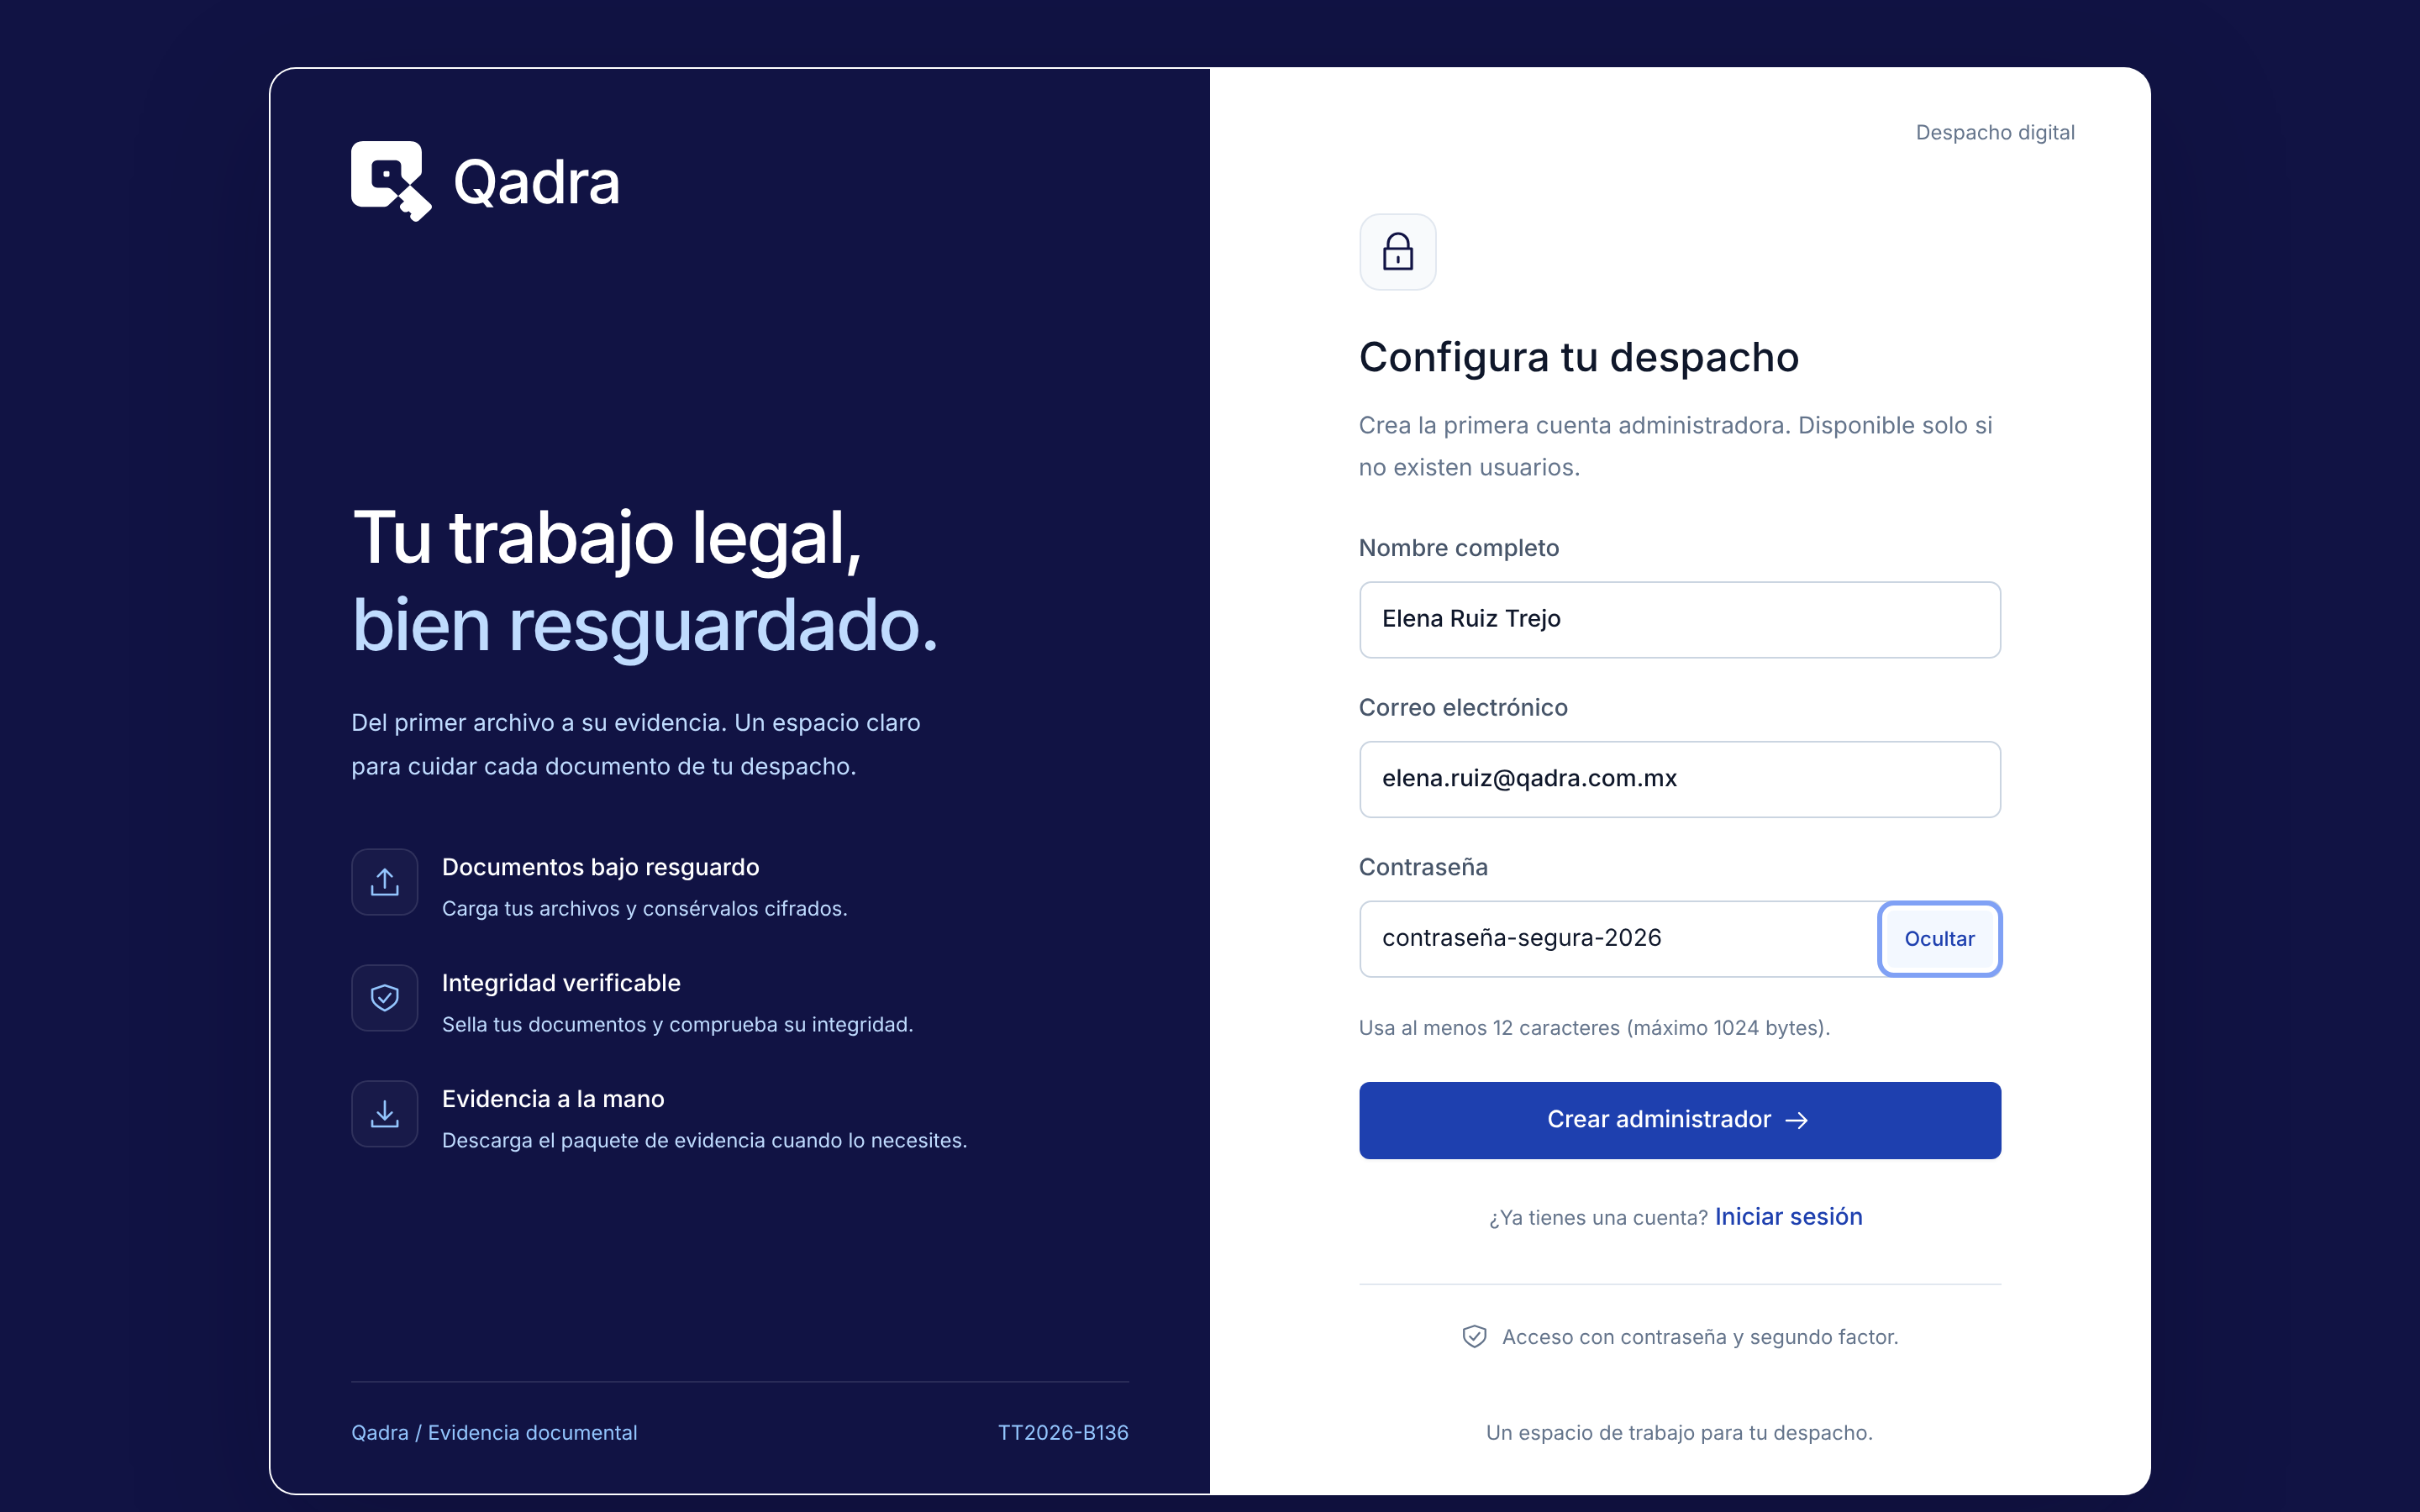
\includegraphics[width=0.9\textwidth]{capturas/A-01-configurar-despacho.png}
  \caption{Creación de la primera cuenta de Administrador.}
  \label{fig:manual-configurar-despacho}
\end{figure}

\begin{figure}[H]
  \centering
  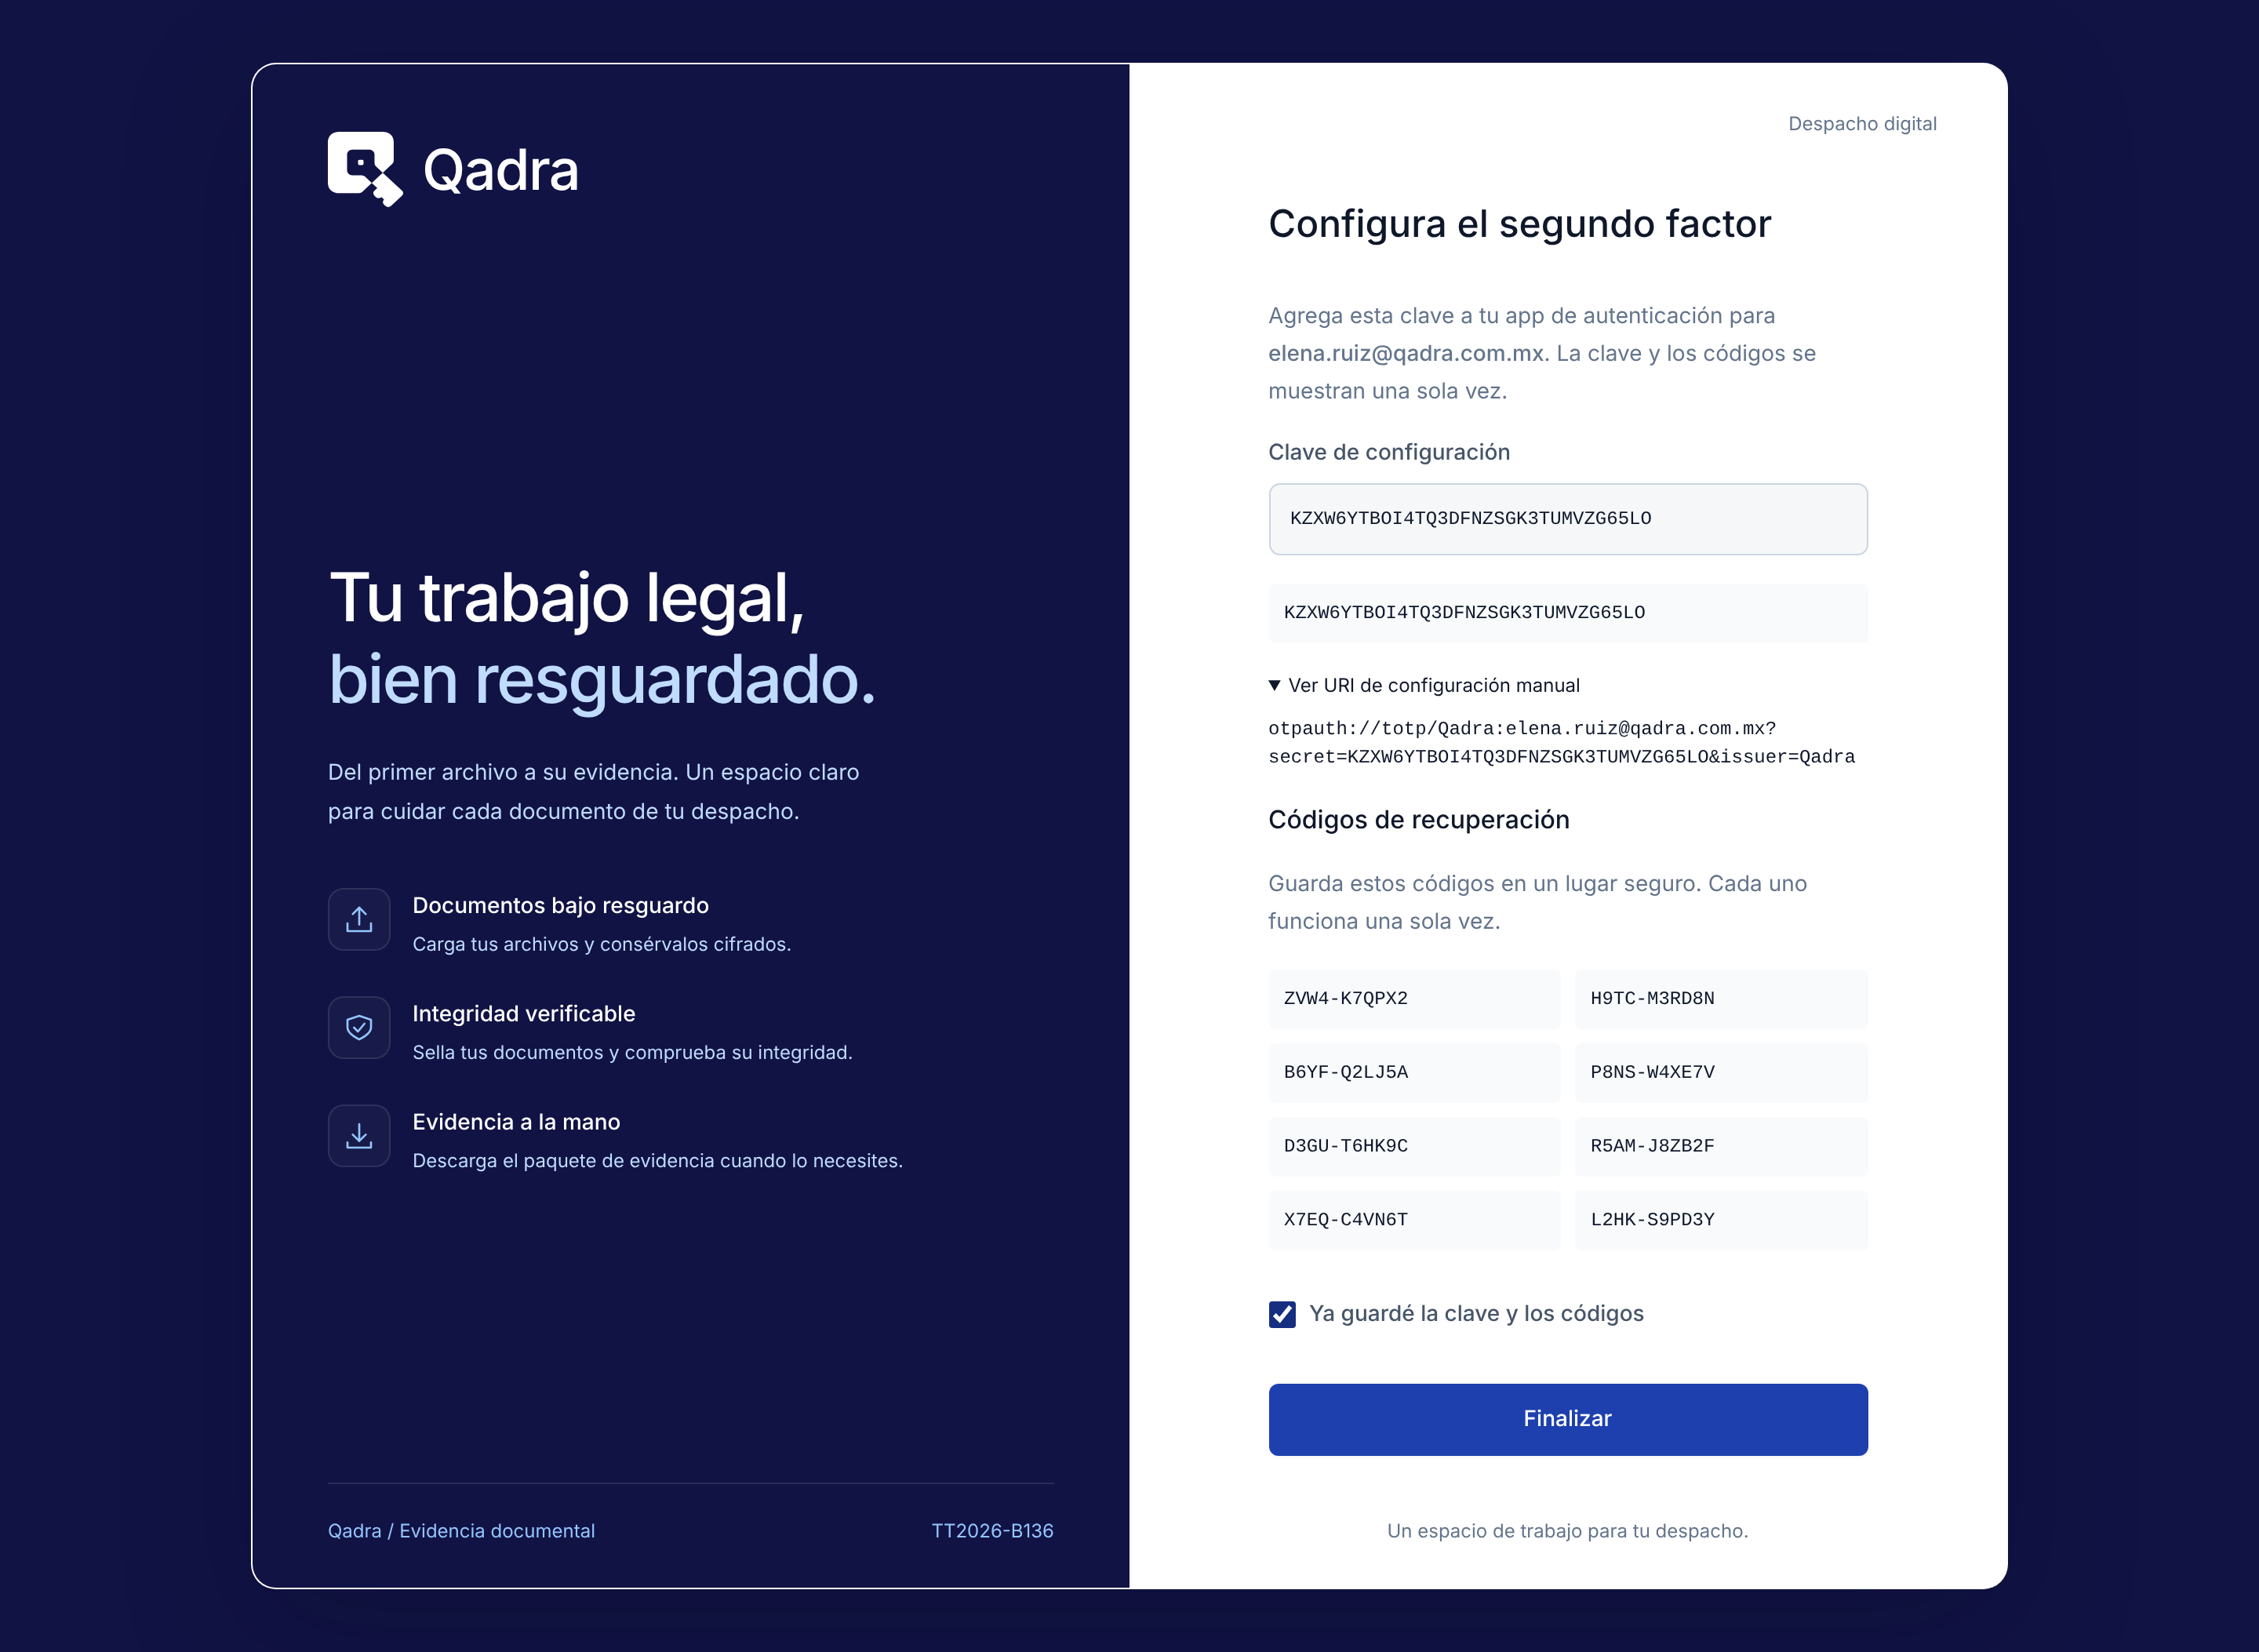
\includegraphics[width=0.9\textwidth]{capturas/A-02-configurar-segundo-factor.png}
  \caption{Configuración del segundo factor y códigos de recuperación.}
  \label{fig:manual-configurar-segundo-factor}
\end{figure}

\resultado La cuenta queda creada y Qadra vuelve a la pantalla de inicio de
sesión. Entre con su correo, su contraseña y su código
(\cref{sec:iniciar-sesion}).

\importante{La clave y los códigos se muestran una sola vez. Guárdelos antes
de hacer clic en \textbf{Finalizar}.}

\nota{Si el despacho ya tiene un Administrador, aparece el mensaje
\enquote{El despacho ya tiene un administrador. Inicia sesión con tu
cuenta.}}

% ---------------------------------------------------------------------
\section{Aceptar una invitación}\label{sec:aceptar-invitacion}

\paraque Crea su cuenta a partir del correo de invitación que le envió el
Administrador.

\disponible Cualquier persona invitada: Litigante, Asistente legal o Cliente.

\pasos
\begin{enumerate}
  \item Abra el enlace del correo de invitación. Aparece la pantalla
        \textbf{Acepta tu invitación}.
  \item En \textbf{Tu contraseña}, escriba la contraseña que usará en Qadra
        (entre 12 y 1024 bytes; en la práctica, al menos 12 caracteres).
  \item Haga clic en \textbf{Preparar segundo factor}.
  \item En la pantalla \textbf{Confirma tu segundo factor}, agregue a su app
        de autenticación la clave que se muestra. Si su app pide un enlace,
        abra \textbf{Enlace para tu autenticador}.
  \item Guarde en un lugar privado los códigos de recuperación de la lista.
  \item Marque la casilla \textbf{Ya guardé mis códigos de recuperación}.
  \item Escriba de nuevo su contraseña en \textbf{Tu contraseña} y el
        \textbf{Código de 6 dígitos} que muestra su app.
  \item Haga clic en \textbf{Confirmar alta}.
\end{enumerate}

\begin{figure}[H]
  \centering
  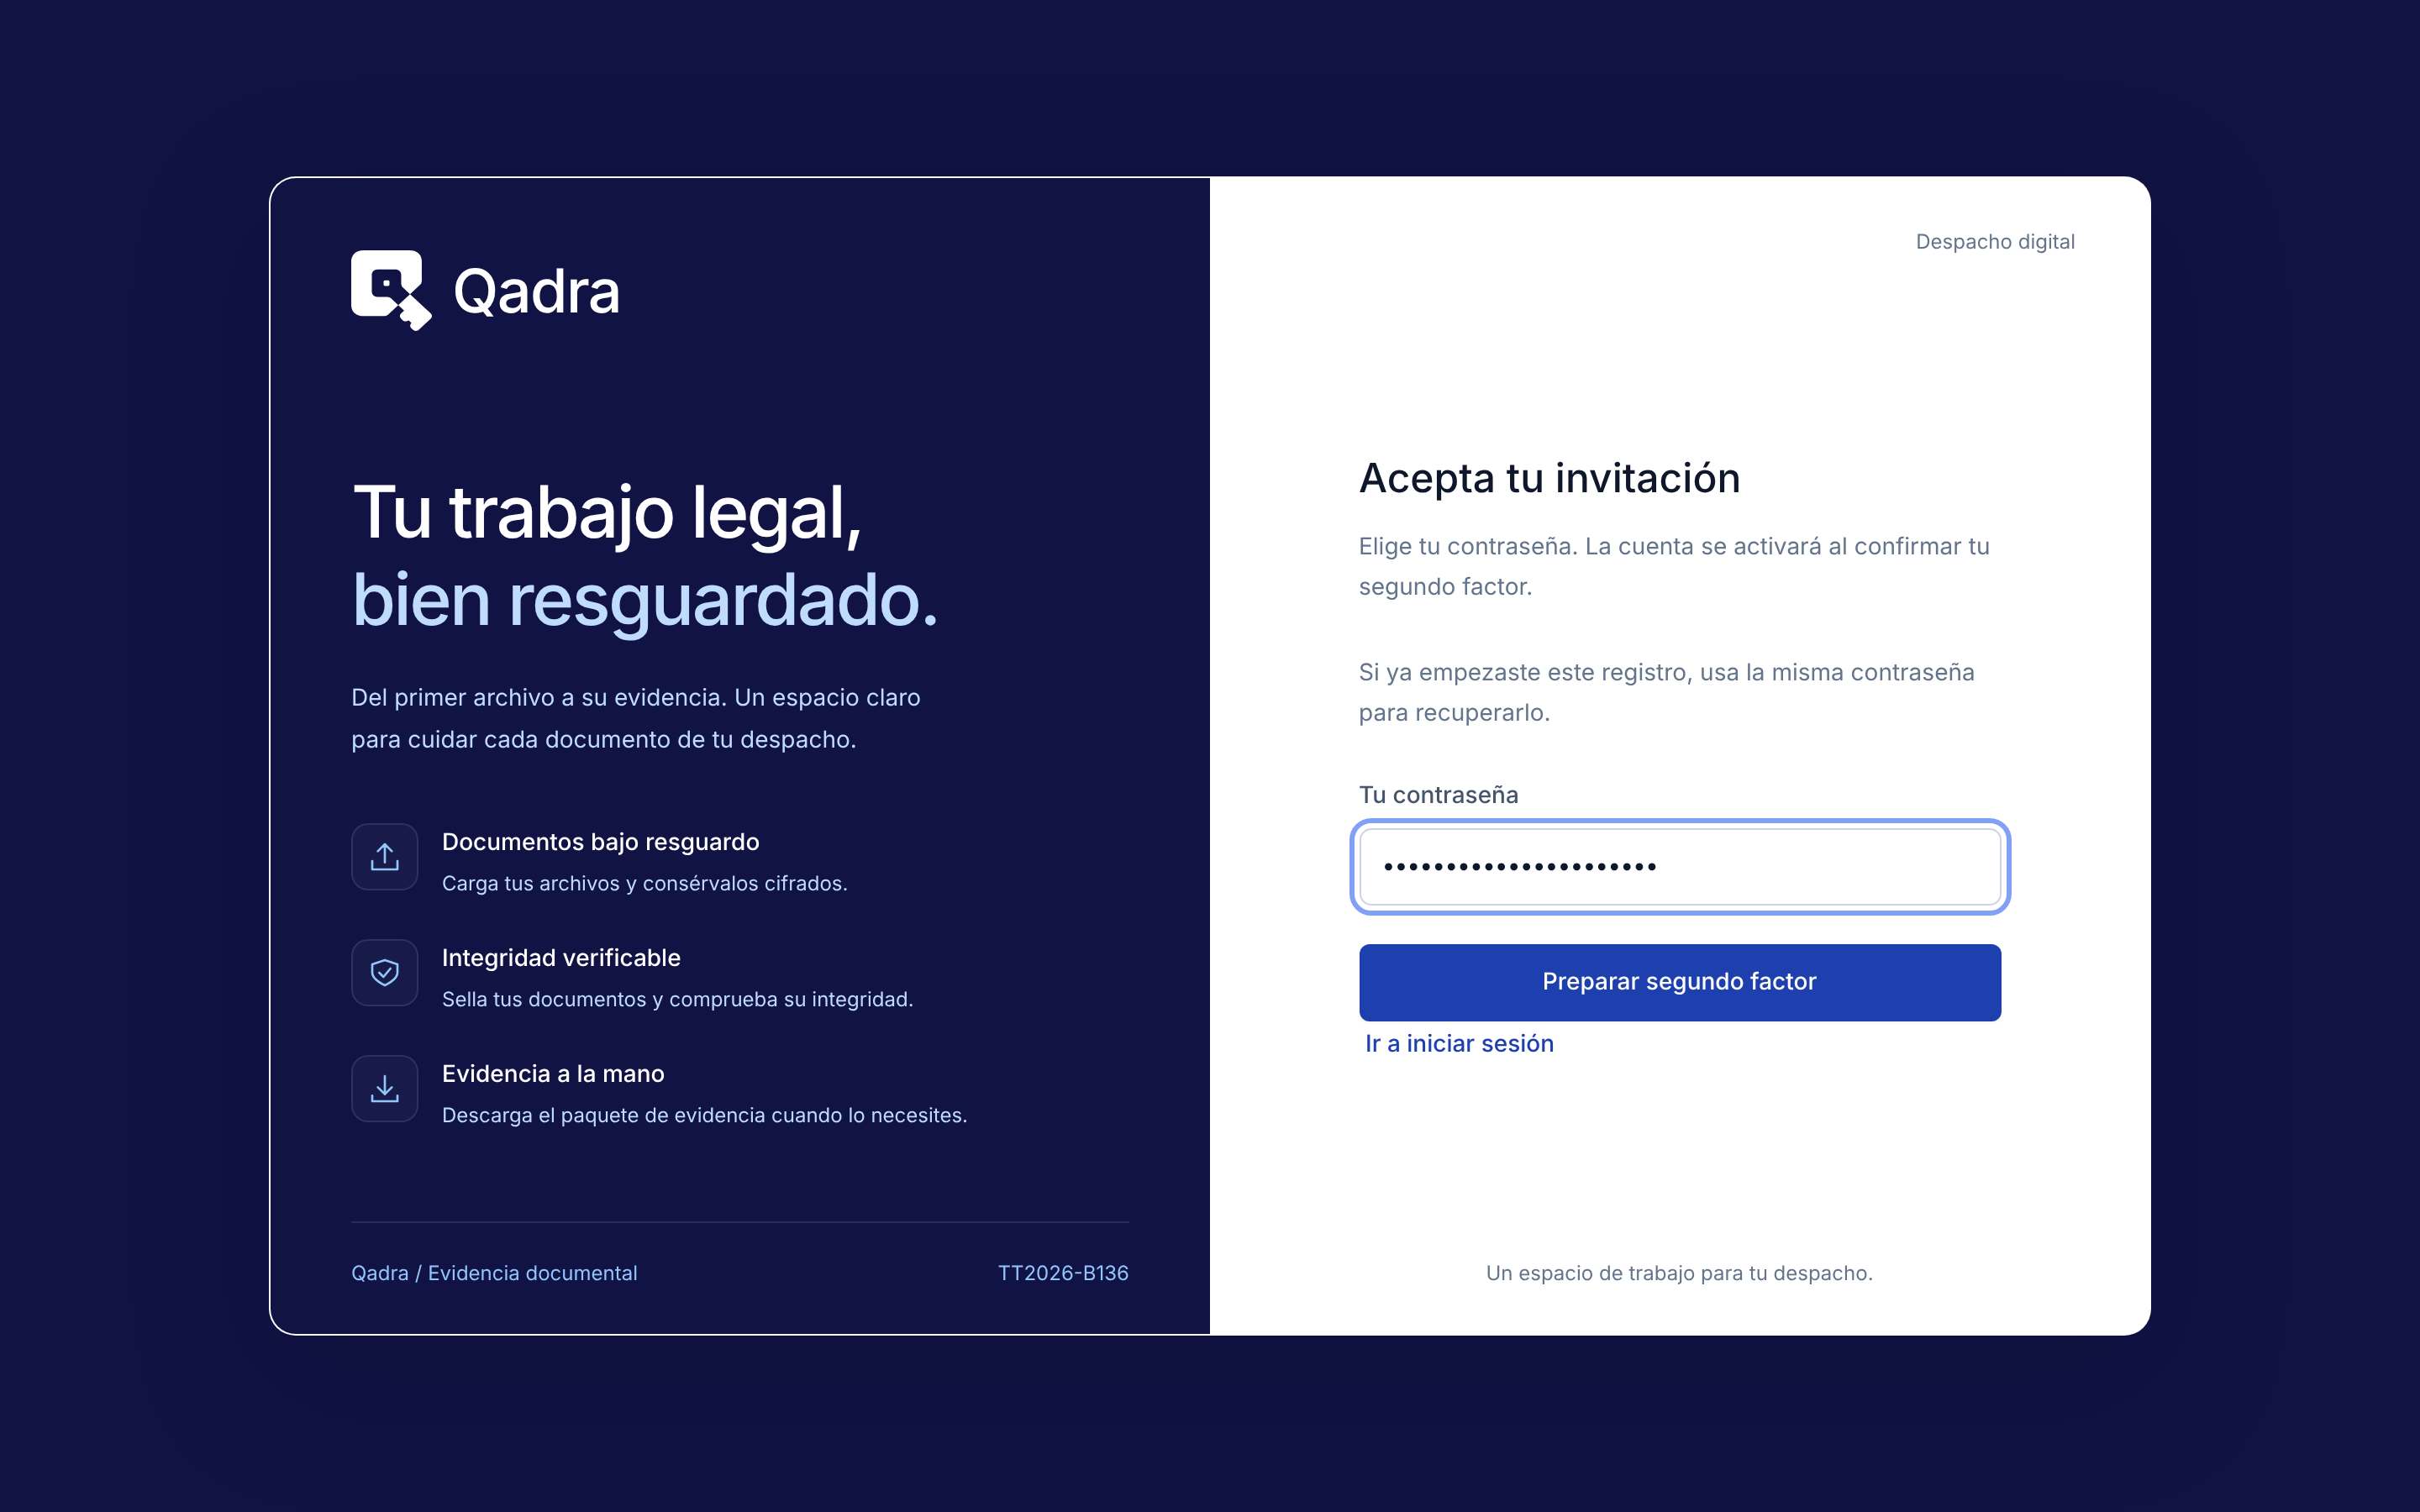
\includegraphics[width=0.9\textwidth]{capturas/A-03-aceptar-invitacion.png}
  \caption{Inicio del alta desde una invitación.}
  \label{fig:manual-aceptar-invitacion}
\end{figure}

\begin{figure}[H]
  \centering
  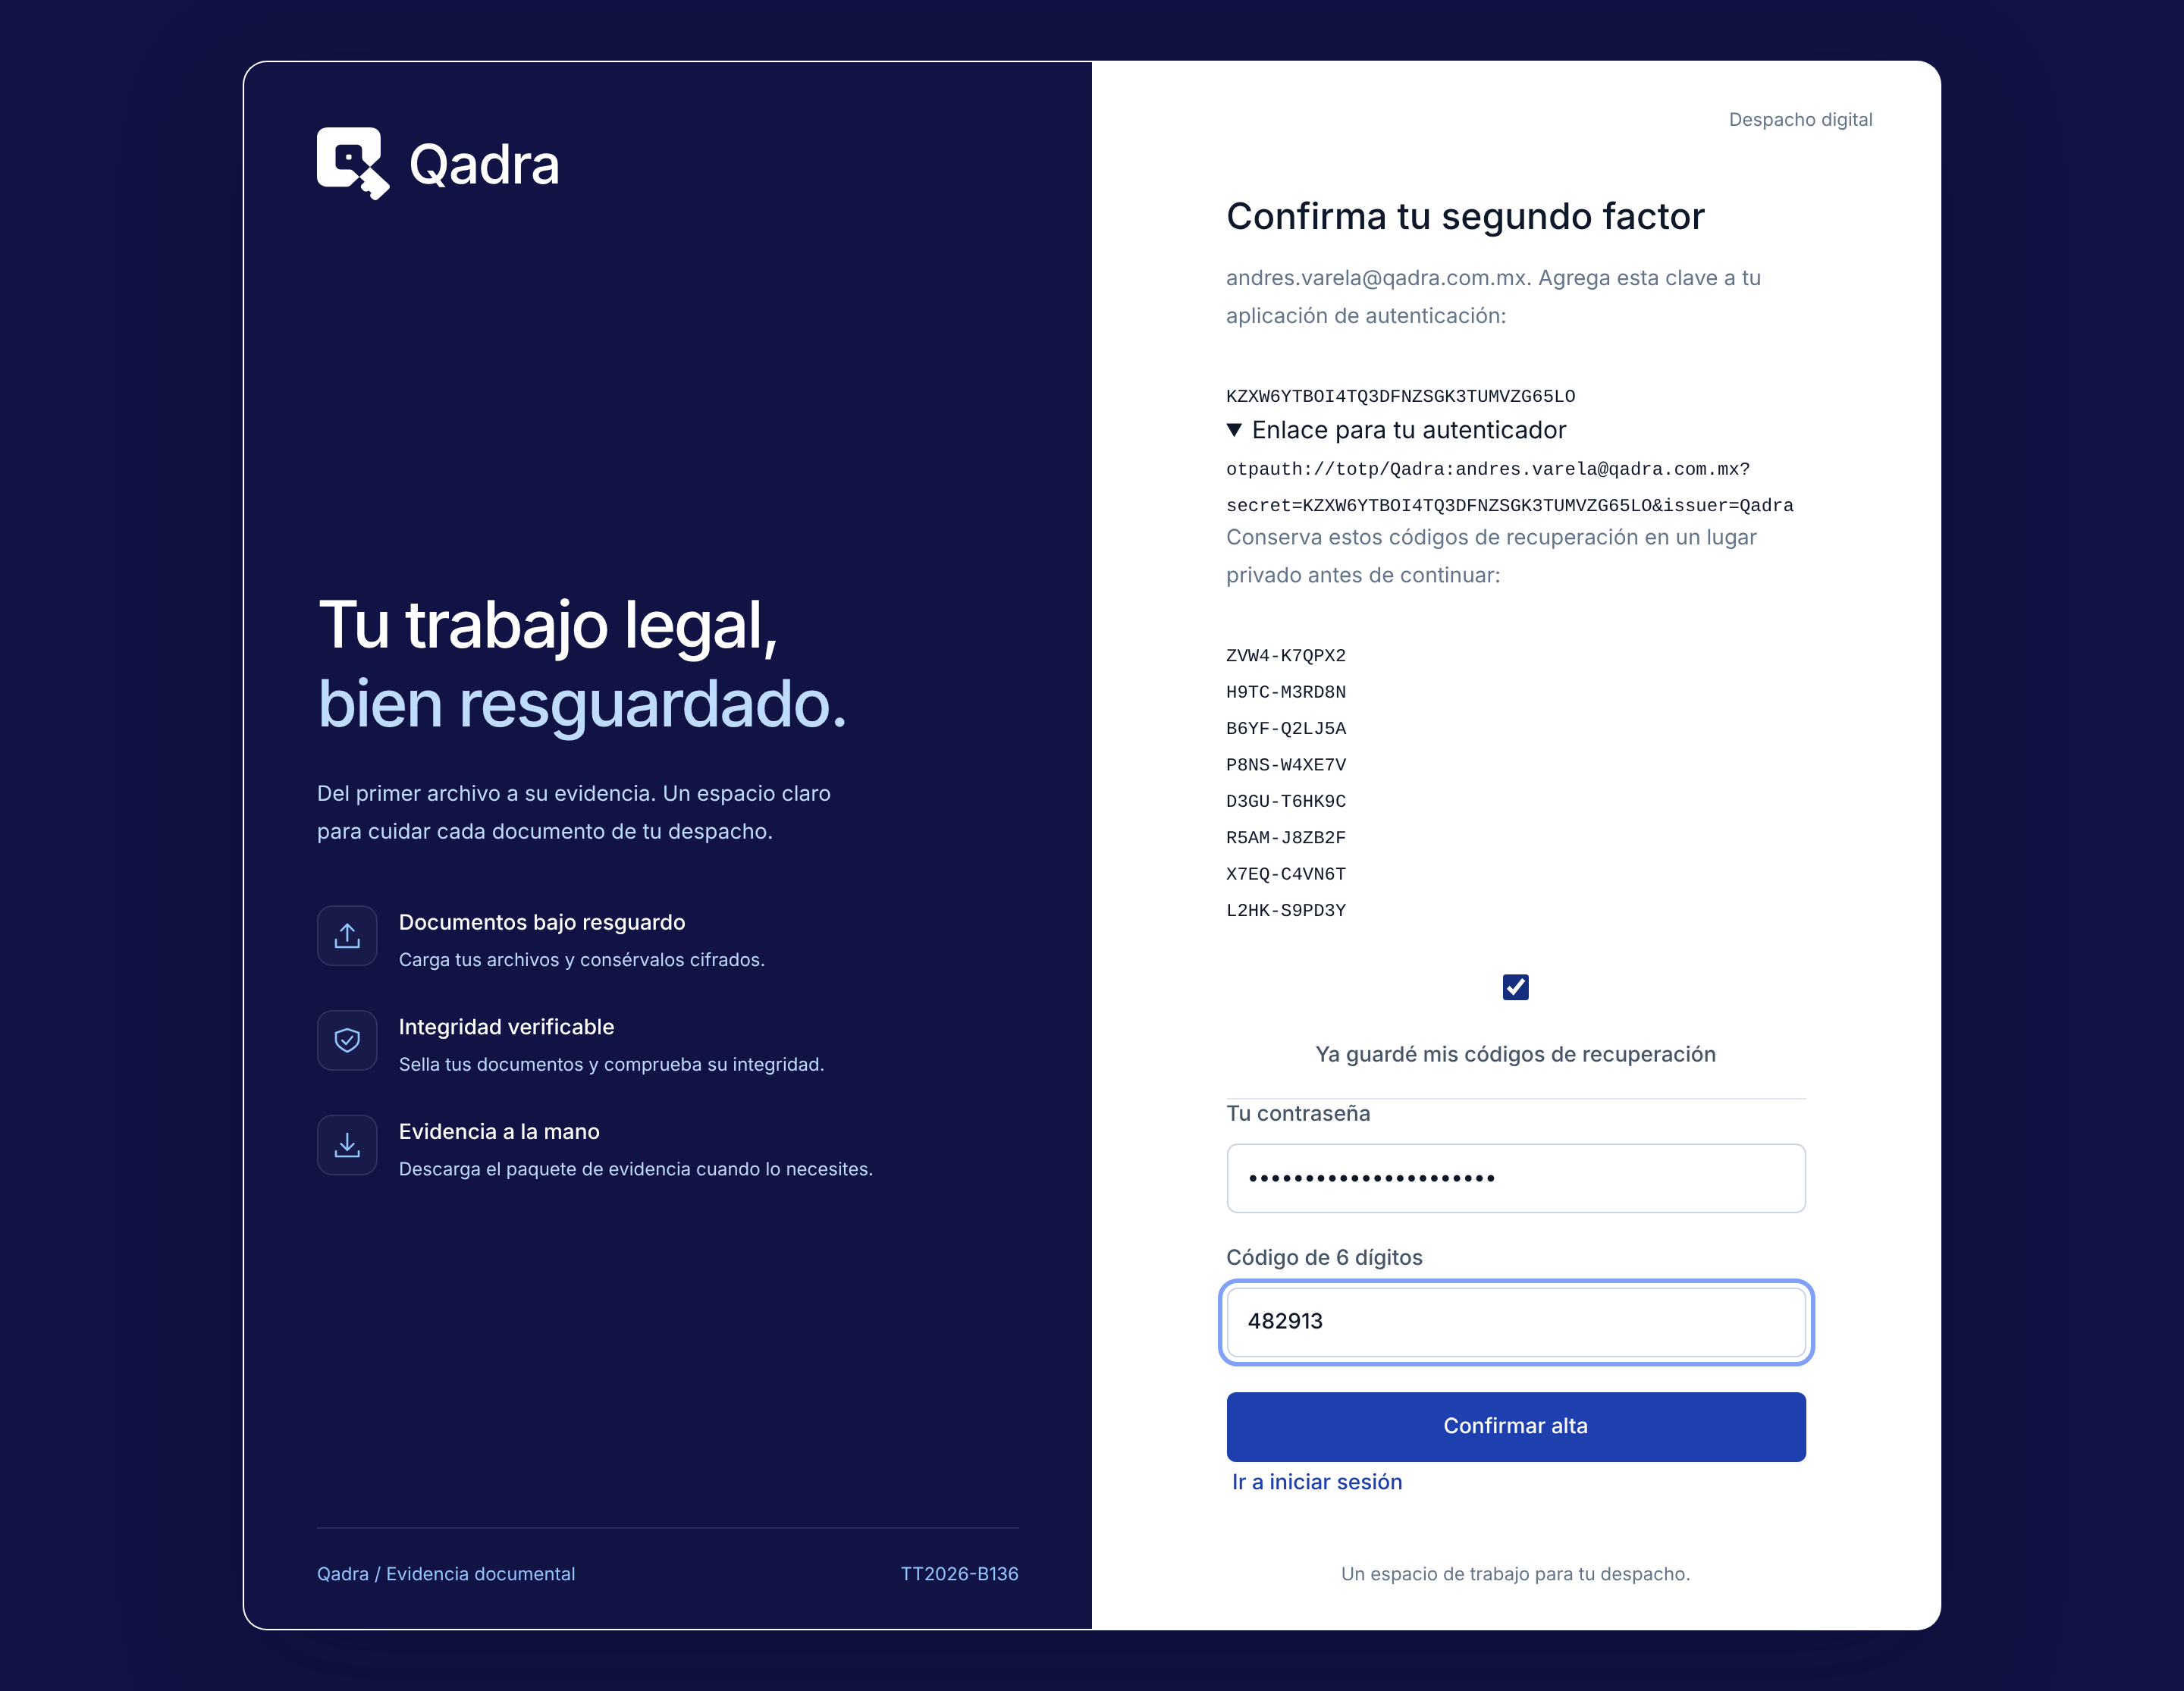
\includegraphics[width=0.9\textwidth]{capturas/A-04-confirmar-segundo-factor.png}
  \caption{Confirmación del segundo factor durante el alta.}
  \label{fig:manual-confirmar-segundo-factor}
\end{figure}

\resultado Aparece \enquote{Cuenta creada: [correo]. Ya puedes iniciar sesión
con tu contraseña y segundo factor.} Haga clic en
\textbf{Ir a iniciar sesión}.

\begin{itemize}
  \item \textbf{Si el alta se interrumpió:} abra de nuevo el mismo enlace.
        Qadra le pide \enquote{Comprueba si tu alta terminó antes de
        repetirla.} Escriba la misma contraseña y haga clic en
        \textbf{Comprobar resultado}.
  \item \textbf{Si el enlace no funciona:} aparece \enquote{El enlace no es
        válido. Abre el correo original o solicita un reenvío al
        administrador.}
  \item \textbf{Si el navegador no puede guardar el intento:} se le pide
        conservar la pestaña abierta hasta confirmar el alta. No la cierre.
\end{itemize}

% ---------------------------------------------------------------------
\section{Iniciar sesión}\label{sec:iniciar-sesion}

\paraque Permite entrar a Qadra con su correo, su contraseña y el código de
su app de autenticación.

\disponible Todos los roles con cuenta.

\pasos
\begin{enumerate}
  \item Abra Qadra en su navegador. Aparece la pantalla
        \textbf{Accede a tu despacho}.
  \item Ingrese su \textbf{Correo electrónico} y su \textbf{Contraseña}.
        Para revisar lo que escribió, haga clic en \textbf{Mostrar}.
  \item Haga clic en \textbf{Continuar}.
  \item En la pantalla \textbf{Un paso más}, abra su app de autenticación y
        escriba el \textbf{Código de 6 dígitos}.
  \item Haga clic en \textbf{Verificar y entrar}.
\end{enumerate}

\begin{figure}[H]
  \centering
  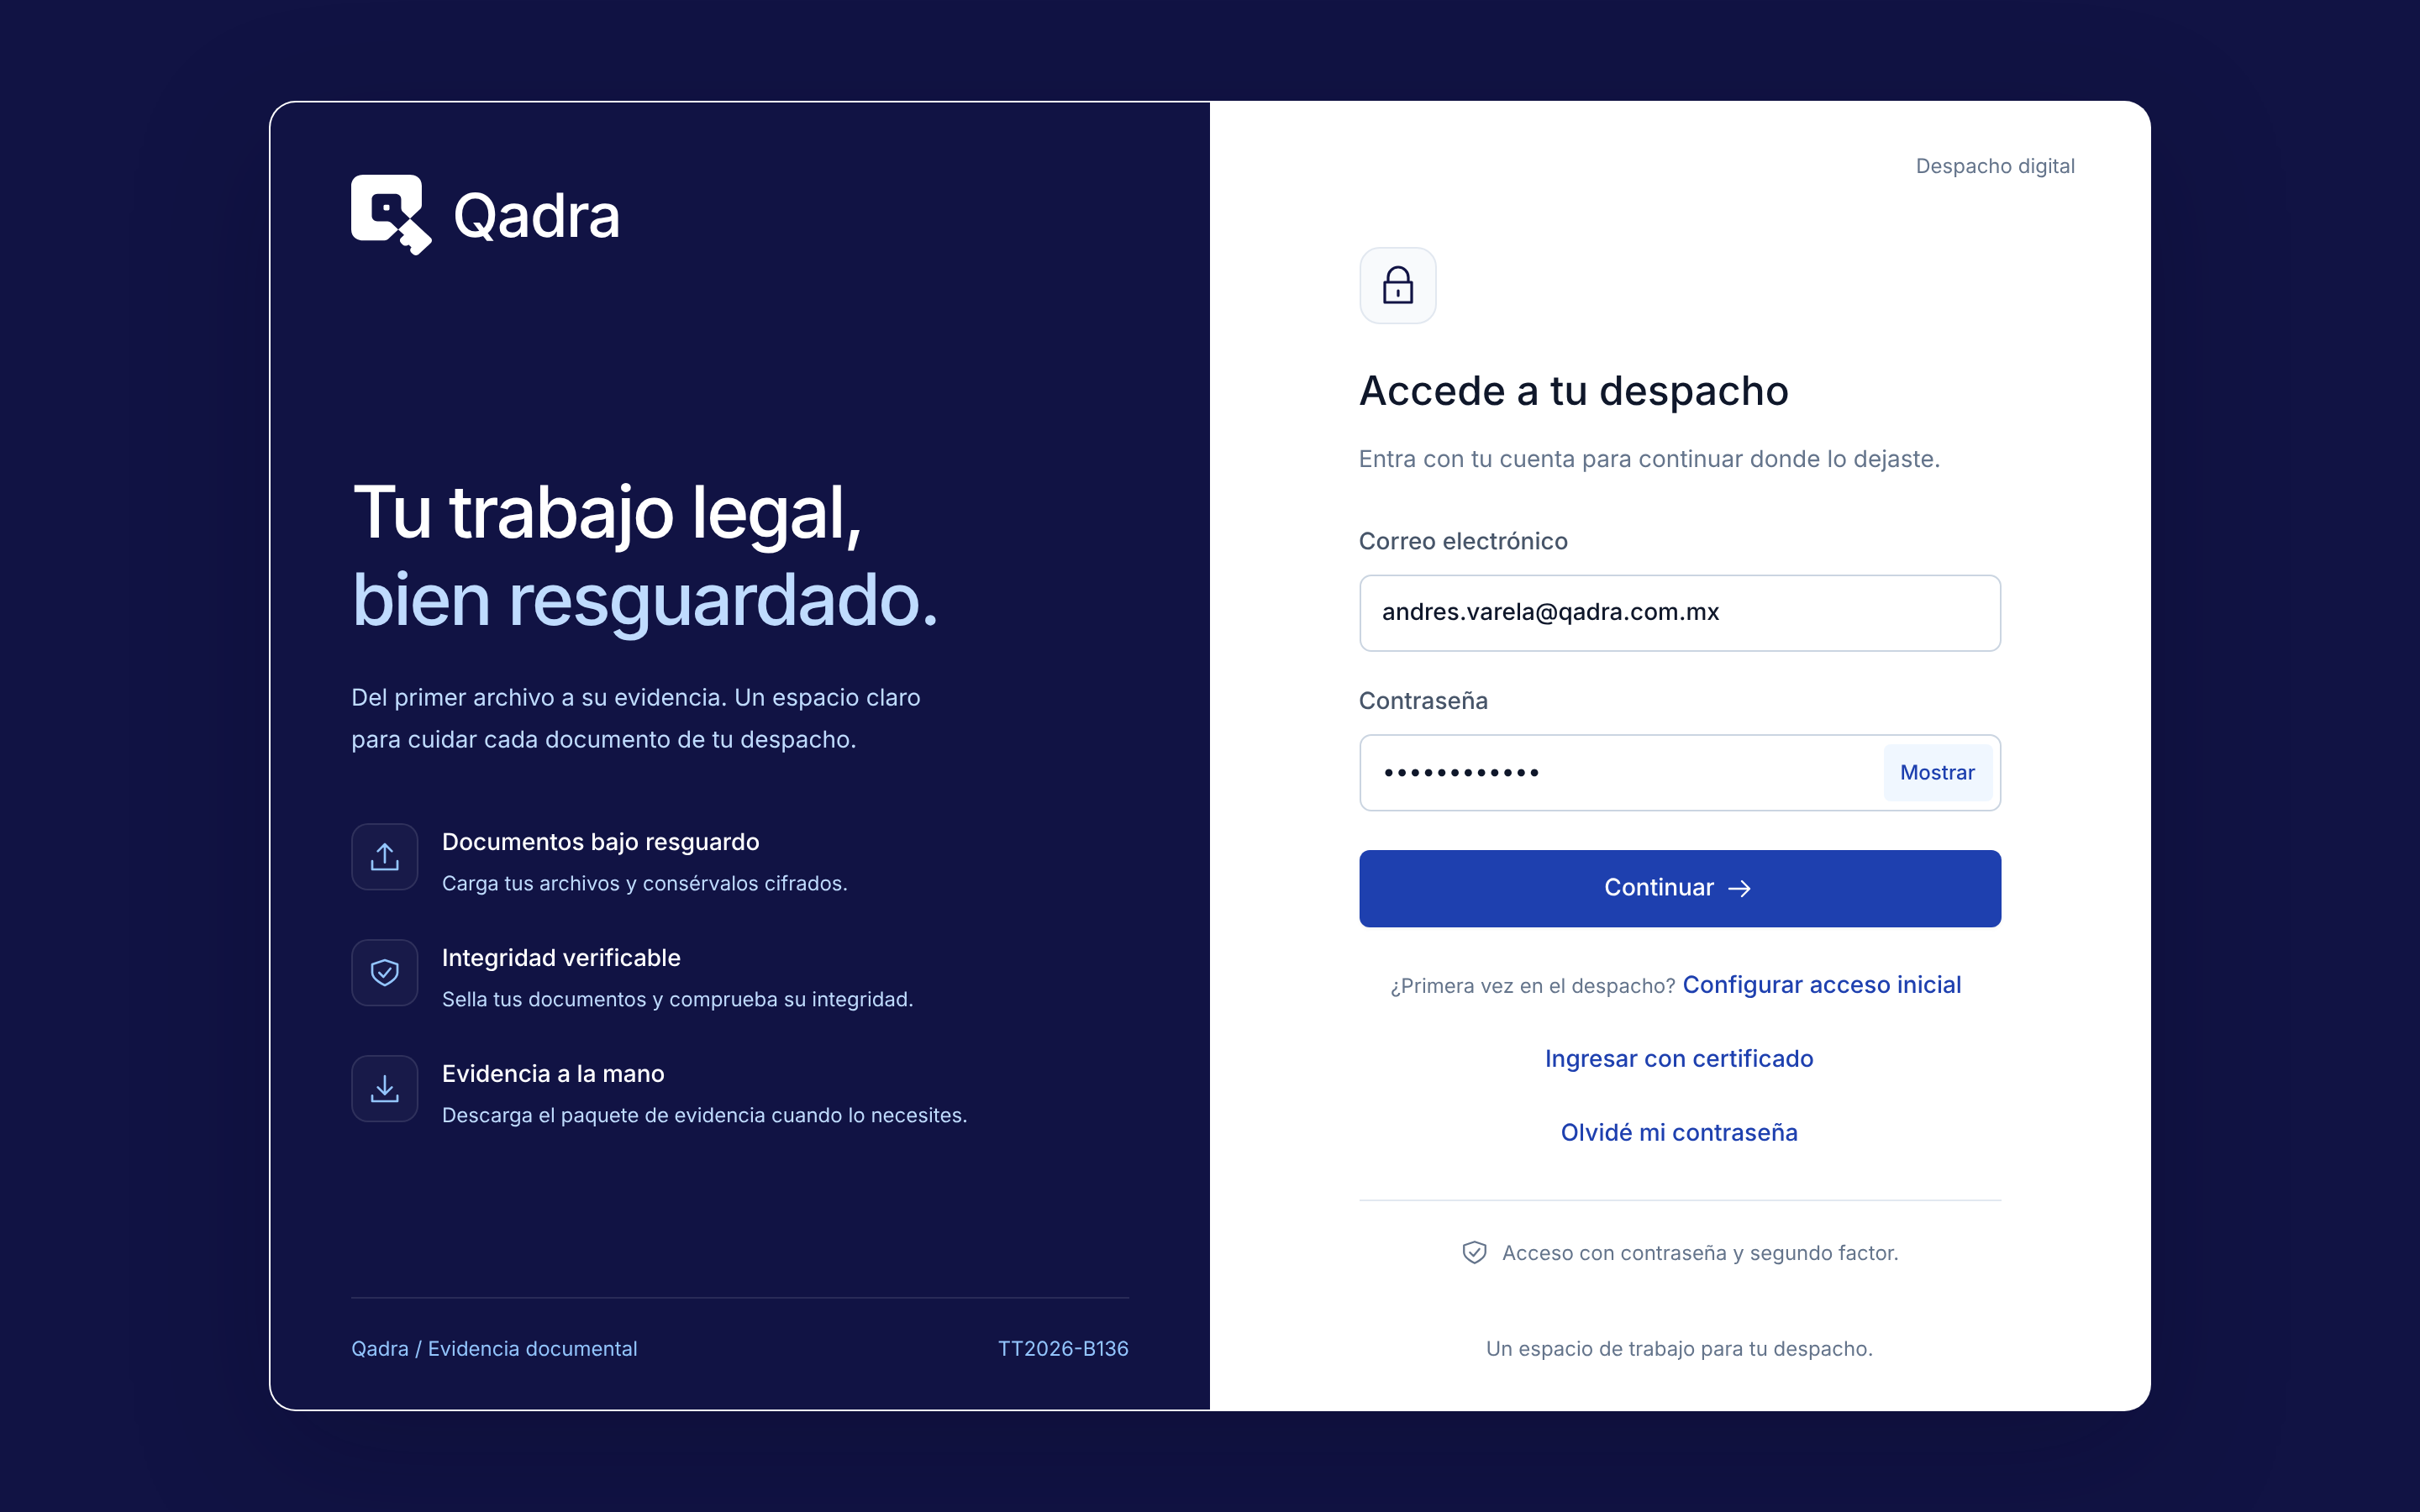
\includegraphics[width=0.9\textwidth]{capturas/A-05-inicio-sesion.png}
  \caption{Inicio de sesión con correo y contraseña.}
  \label{fig:manual-inicio-sesion}
\end{figure}

\begin{figure}[H]
  \centering
  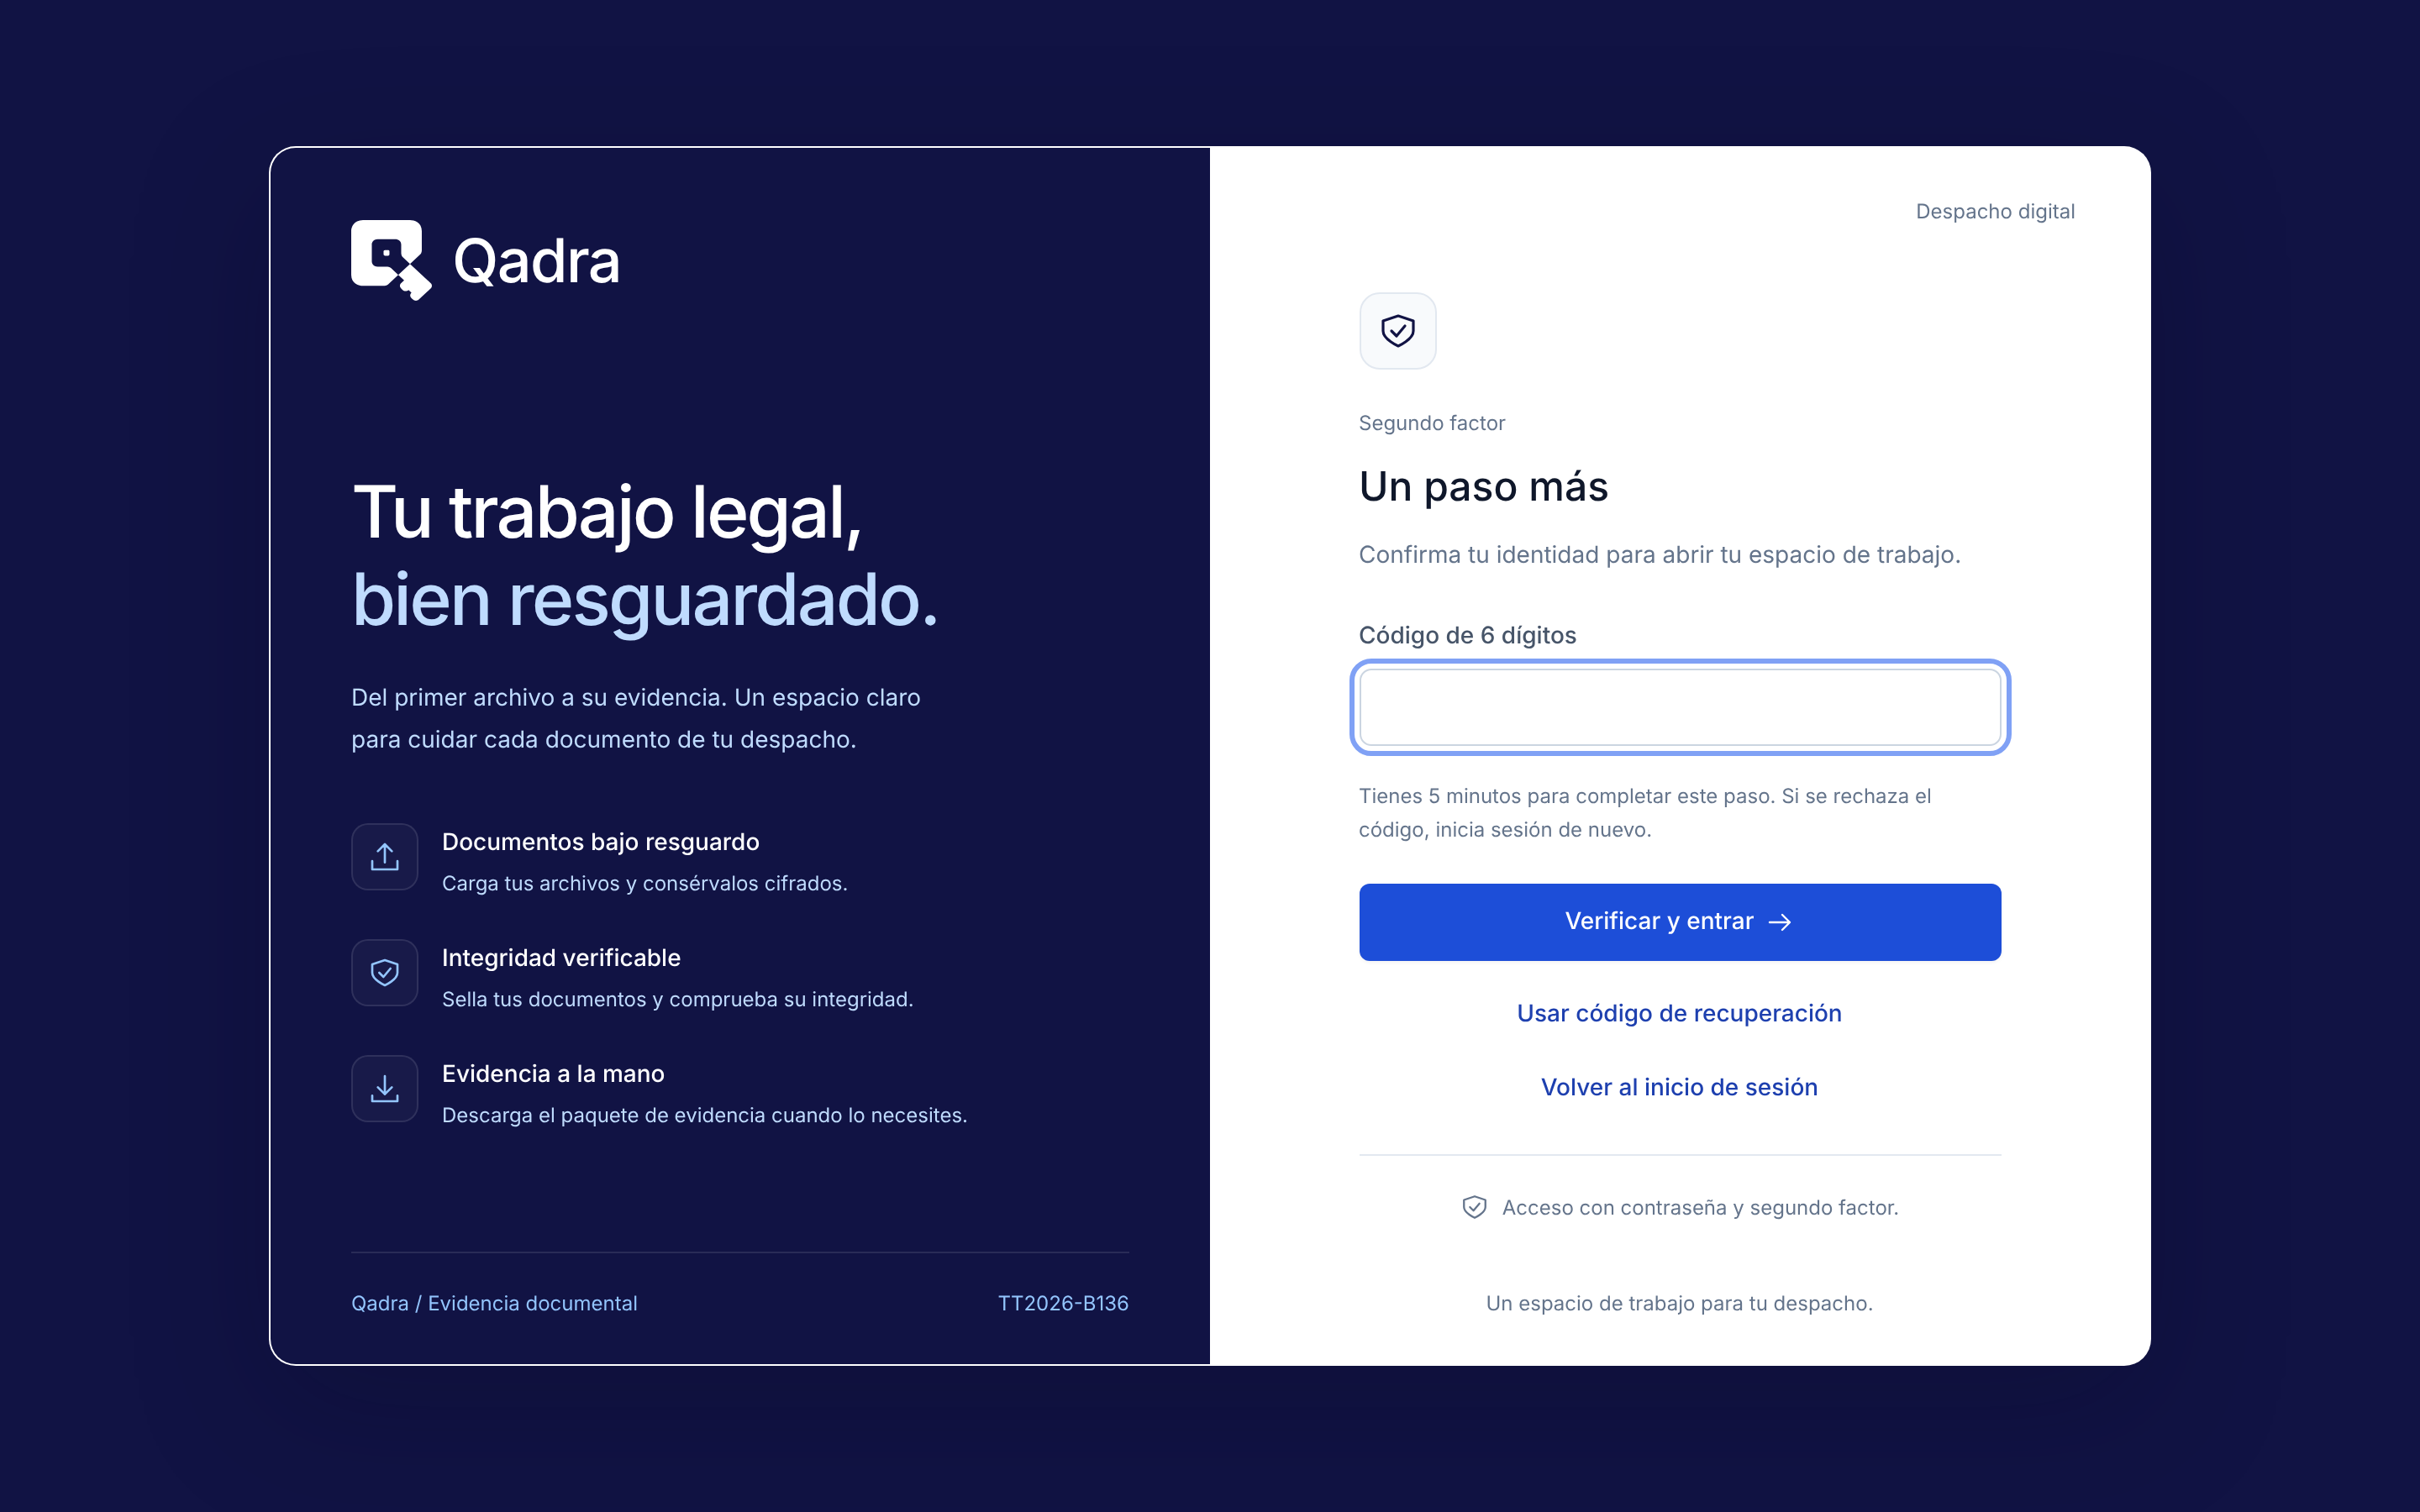
\includegraphics[width=0.9\textwidth]{capturas/A-06-segundo-factor.png}
  \caption{Confirmación con el segundo factor.}
  \label{fig:manual-segundo-factor}
\end{figure}

\resultado Se abre su espacio de trabajo. El Administrador, el Litigante y el
Asistente legal llegan a \textbf{Inicio}; el Cliente llega a
\textbf{Mis contratos}.

\begin{itemize}
  \item La pantalla indica el tiempo disponible para escribir el código:
        \enquote{Tienes 5 minutos para completar este paso. Si se rechaza el código, inicia
        sesión de nuevo.}
  \item Si el código se rechaza, aparece \enquote{El código fue rechazado o
        venció. Vuelve a iniciar sesión.} Empiece de nuevo desde el paso 1.
  \item Después de varios intentos fallidos aparece \enquote{Demasiados
        intentos. Espera 15 minutos antes de volver a intentarlo.}
\end{itemize}

% ---------------------------------------------------------------------
\section{Entrar con un código de recuperación}\label{sec:codigo-recuperacion}

\paraque Permite entrar cuando no tiene a la mano su app de autenticación.

\disponible Todos los roles con cuenta.

\pasos
\begin{enumerate}
  \item Siga los pasos 1 a 3 de la \cref{sec:iniciar-sesion}.
  \item En la pantalla \textbf{Un paso más}, haga clic en
        \textbf{Usar código de recuperación}.
  \item Escriba uno de sus códigos en \textbf{Código de recuperación}.
  \item Haga clic en \textbf{Verificar y entrar}.
\end{enumerate}

\resultado Entra a Qadra como en un inicio de sesión normal.

\nota{Cada código funciona una sola vez; táchelo de su lista después de
usarlo. Si ya no conserva ningún código, contacte al Administrador. Para
volver al código de su app, haga clic en \textbf{Usar app de autenticación}.}

% ---------------------------------------------------------------------
\section{Recuperar la contraseña}\label{sec:recuperar-contrasena}

\paraque Permite elegir una contraseña nueva si olvidó la anterior. Su
segundo factor no cambia.

\disponible Todos los roles con cuenta.

\pasos
\begin{enumerate}
  \item En la pantalla de inicio de sesión, haga clic en
        \textbf{Olvidé mi contraseña}.
  \item En \textbf{Recupera tu acceso.}, ingrese su
        \textbf{Correo electrónico} y haga clic en
        \textbf{Solicitar enlace}.
  \item Abra el enlace que llegue a su correo.
  \item En \textbf{Elige una nueva contraseña.}, escriba la
        \textbf{Nueva contraseña} y repítala en
        \textbf{Repite la nueva contraseña}. Use al menos 12 caracteres y no
        reutilice la anterior.
  \item Haga clic en \textbf{Cambiar contraseña}.
\end{enumerate}

\begin{figure}[H]
  \centering
  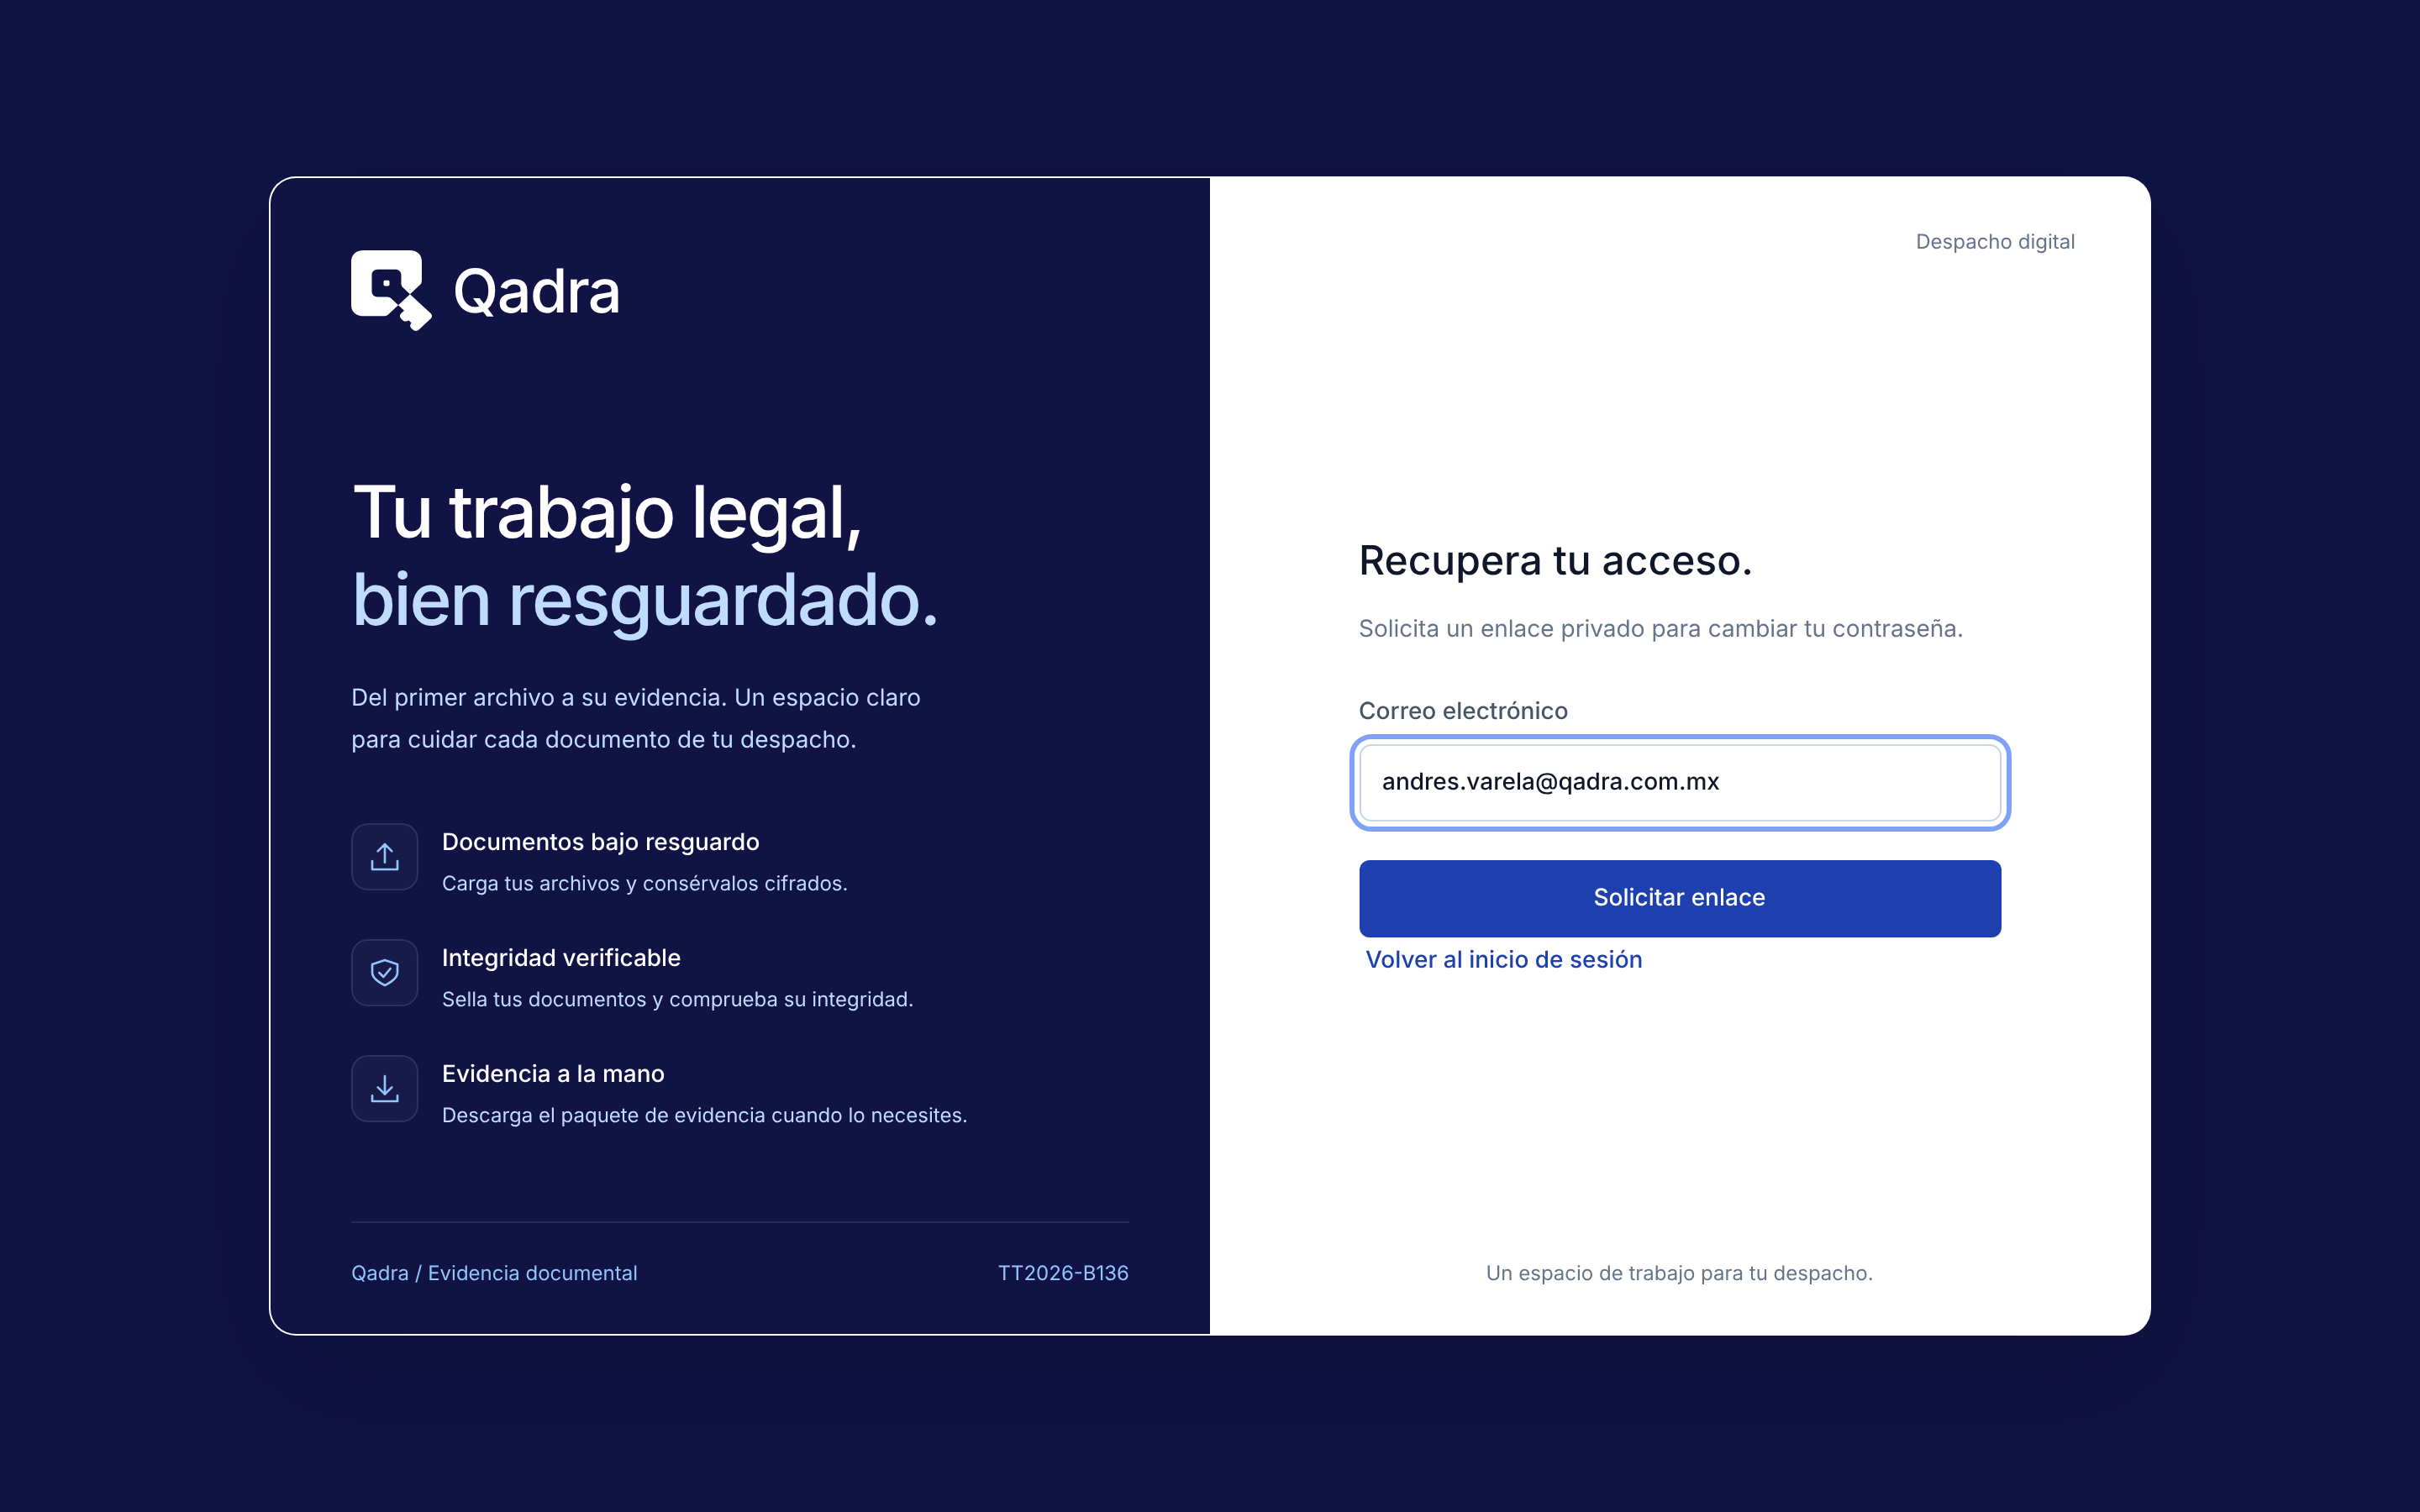
\includegraphics[width=0.9\textwidth]{capturas/A-07-recuperar-acceso.png}
  \caption{Solicitud del enlace de recuperación.}
  \label{fig:manual-recuperar-acceso}
\end{figure}

\begin{figure}[H]
  \centering
  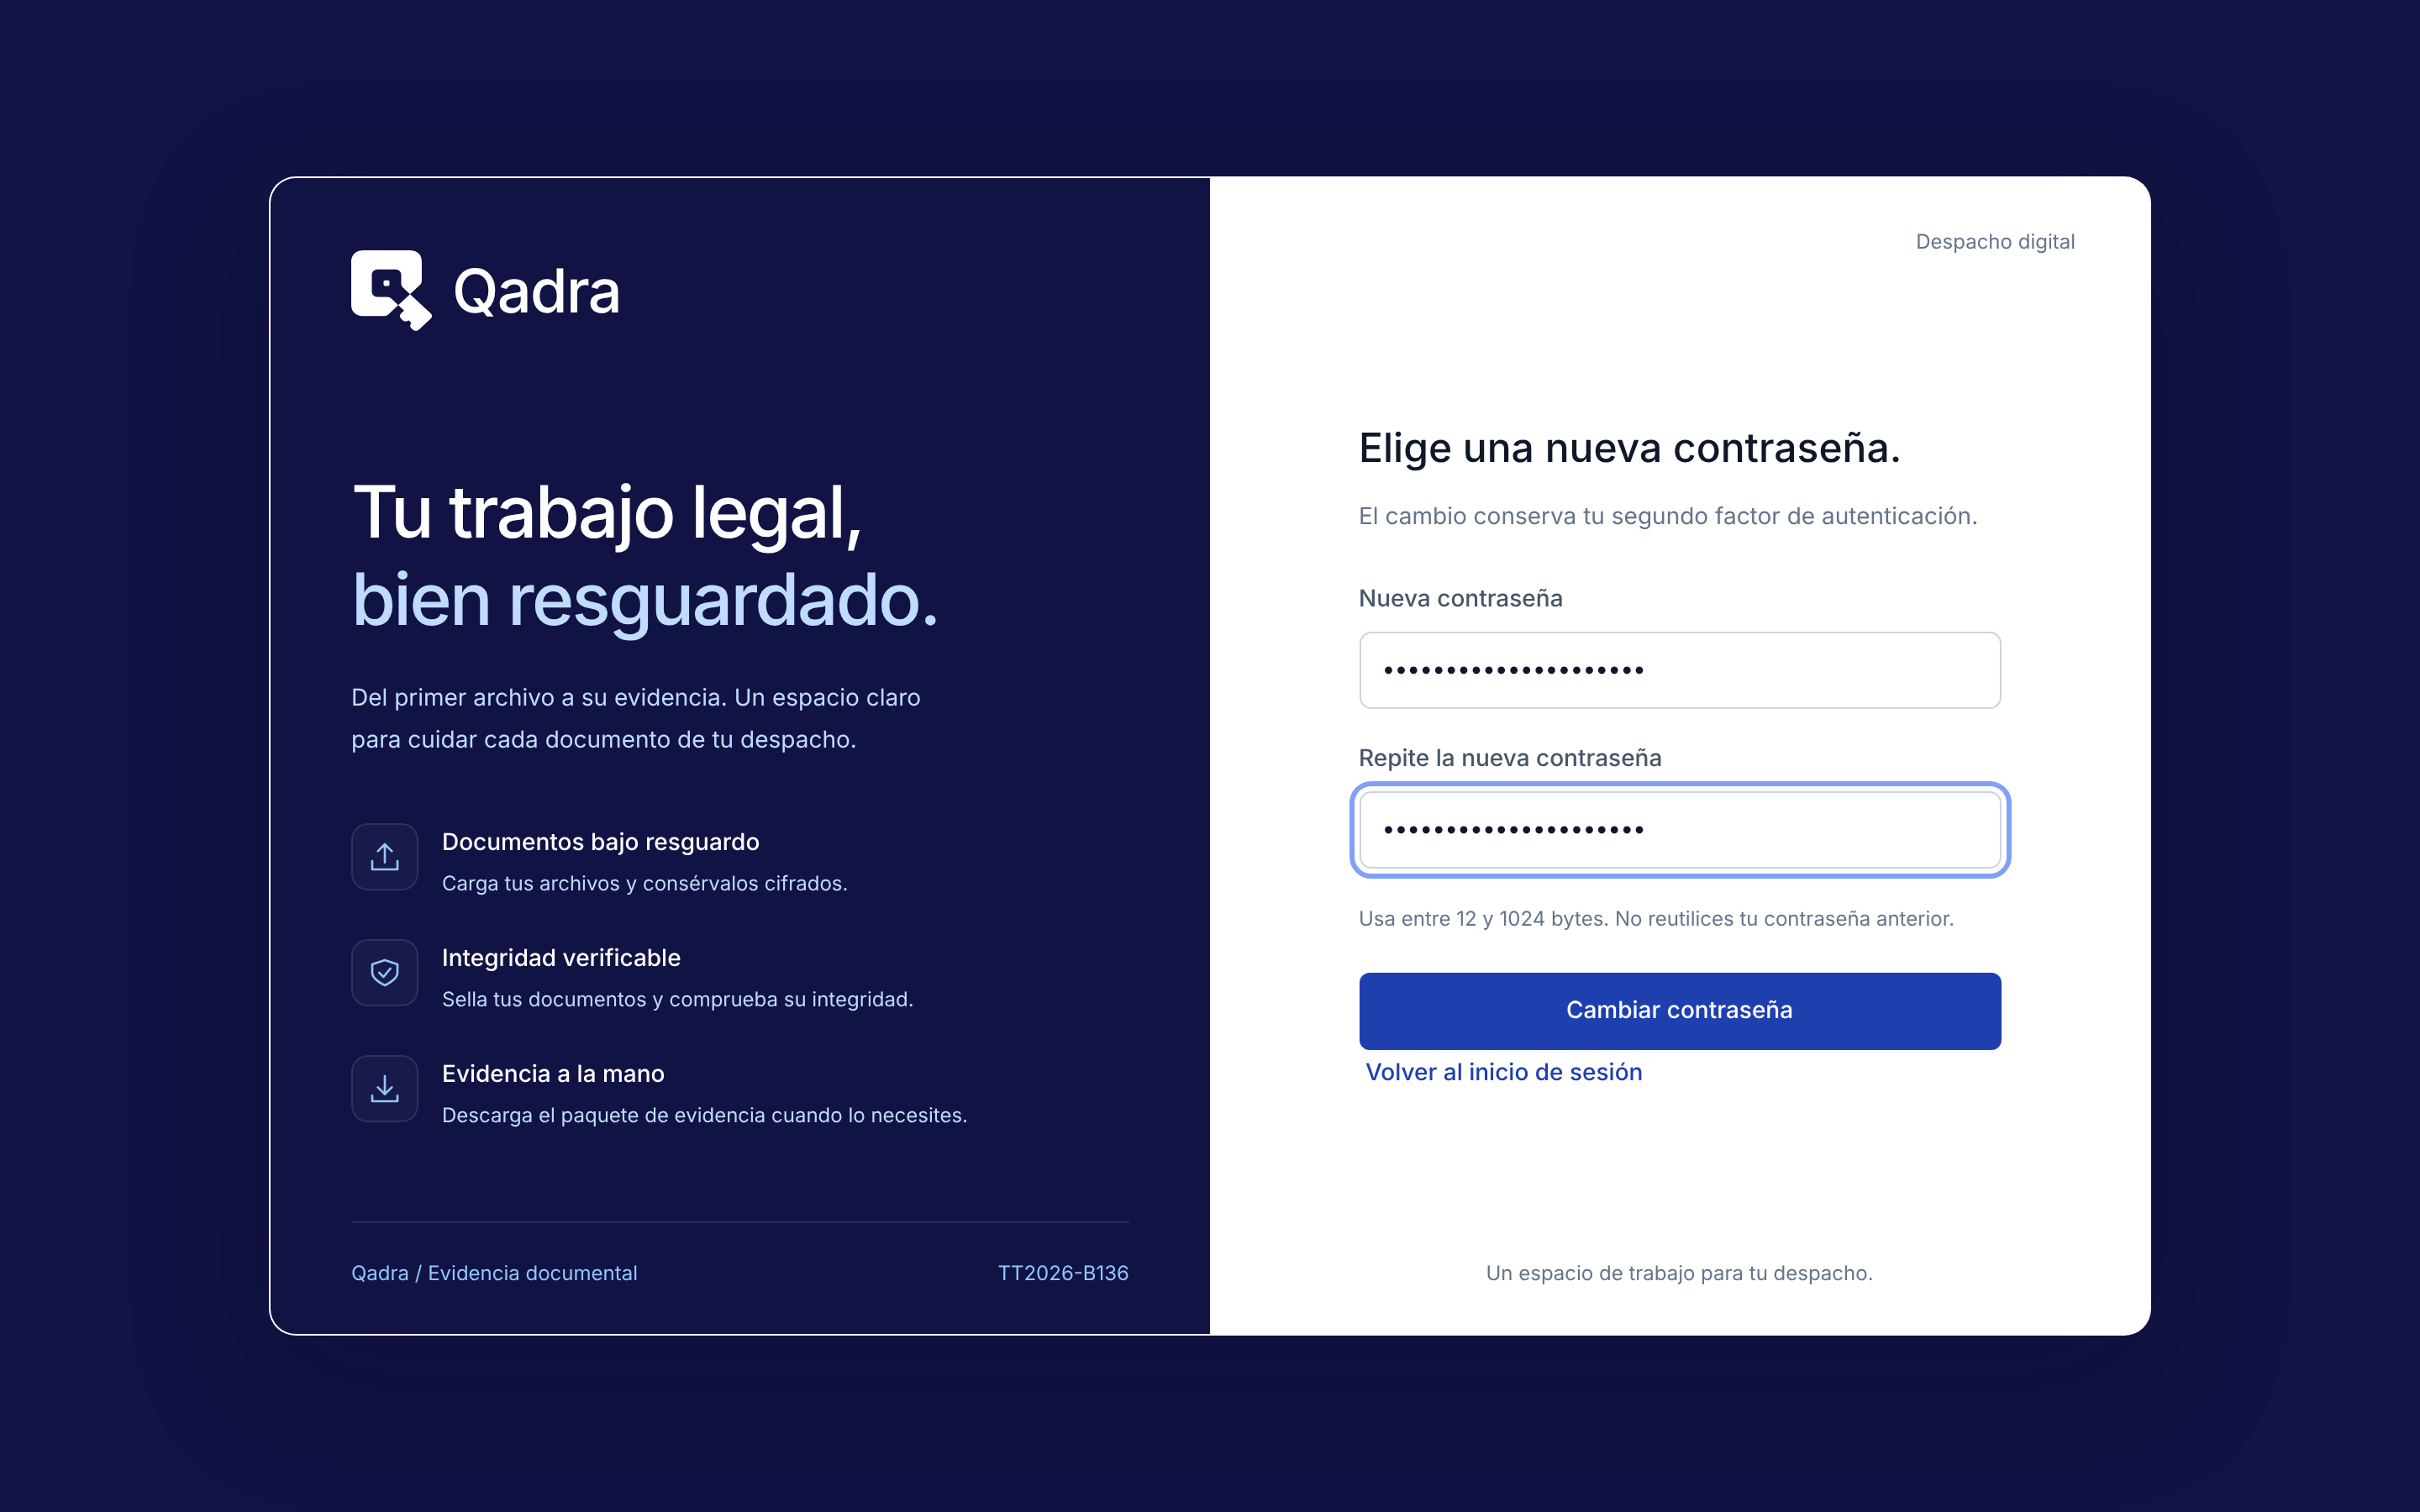
\includegraphics[width=0.9\textwidth]{capturas/A-08-nueva-contrasena.png}
  \caption{Cambio de contraseña desde el enlace.}
  \label{fig:manual-nueva-contrasena}
\end{figure}

\resultado Aparece \enquote{Contraseña actualizada. Inicia sesión con la nueva
contraseña.} Haga clic en \textbf{Volver al inicio de sesión}.

\begin{itemize}
  \item Al solicitar el enlace siempre aparece \enquote{Si la solicitud puede
        atenderse, podrás recibir un enlace. Esta respuesta no confirma un
        envío.} Si no llega ningún correo, revise la dirección escrita o
        contacte al Administrador.
  \item Si el enlace ya se usó o venció, aparece \enquote{El enlace ya no
        puede usarse. Solicita uno nuevo desde el inicio de sesión.}
\end{itemize}

% ---------------------------------------------------------------------
\section{Ingresar con certificado}\label{sec:ingresar-certificado}

\paraque Permite al Administrador entrar con su certificado en lugar de su
contraseña. Después se pide igualmente el segundo factor.

\disponible Administrador, con un certificado vinculado previamente en
\textbf{Mi firma digital}, pestaña \textbf{Acceso con certificado}.

Tenga a la mano: el recibo del vínculo (archivo \texttt{.json}), su clave
privada cifrada (archivo \texttt{.pem}) y la contraseña de esa clave.

\pasos
\begin{enumerate}
  \item En la pantalla de inicio de sesión, haga clic en
        \textbf{Ingresar con certificado}.
  \item En \textbf{Ingresa con tu certificado.}, seleccione su archivo en
        \textbf{Recibo público del vínculo}. Revise que el nombre y la huella
        mostrados sean los suyos.
  \item Haga clic en \textbf{Preparar acceso}.
  \item En \textbf{Firmar en este dispositivo}, seleccione su
        \textbf{Clave privada cifrada} y escriba la
        \textbf{Contraseña de la clave}. Si se solicita, seleccione también
        su certificado en \textbf{Certificado para firma local}.
  \item Haga clic en \textbf{Firmar localmente}.
  \item Haga clic en \textbf{Comprobar firma}.
  \item Escriba el \textbf{Código de 6 dígitos} de su app y haga clic en
        \textbf{Verificar y entrar}.
\end{enumerate}

\begin{figure}[H]
  \centering
  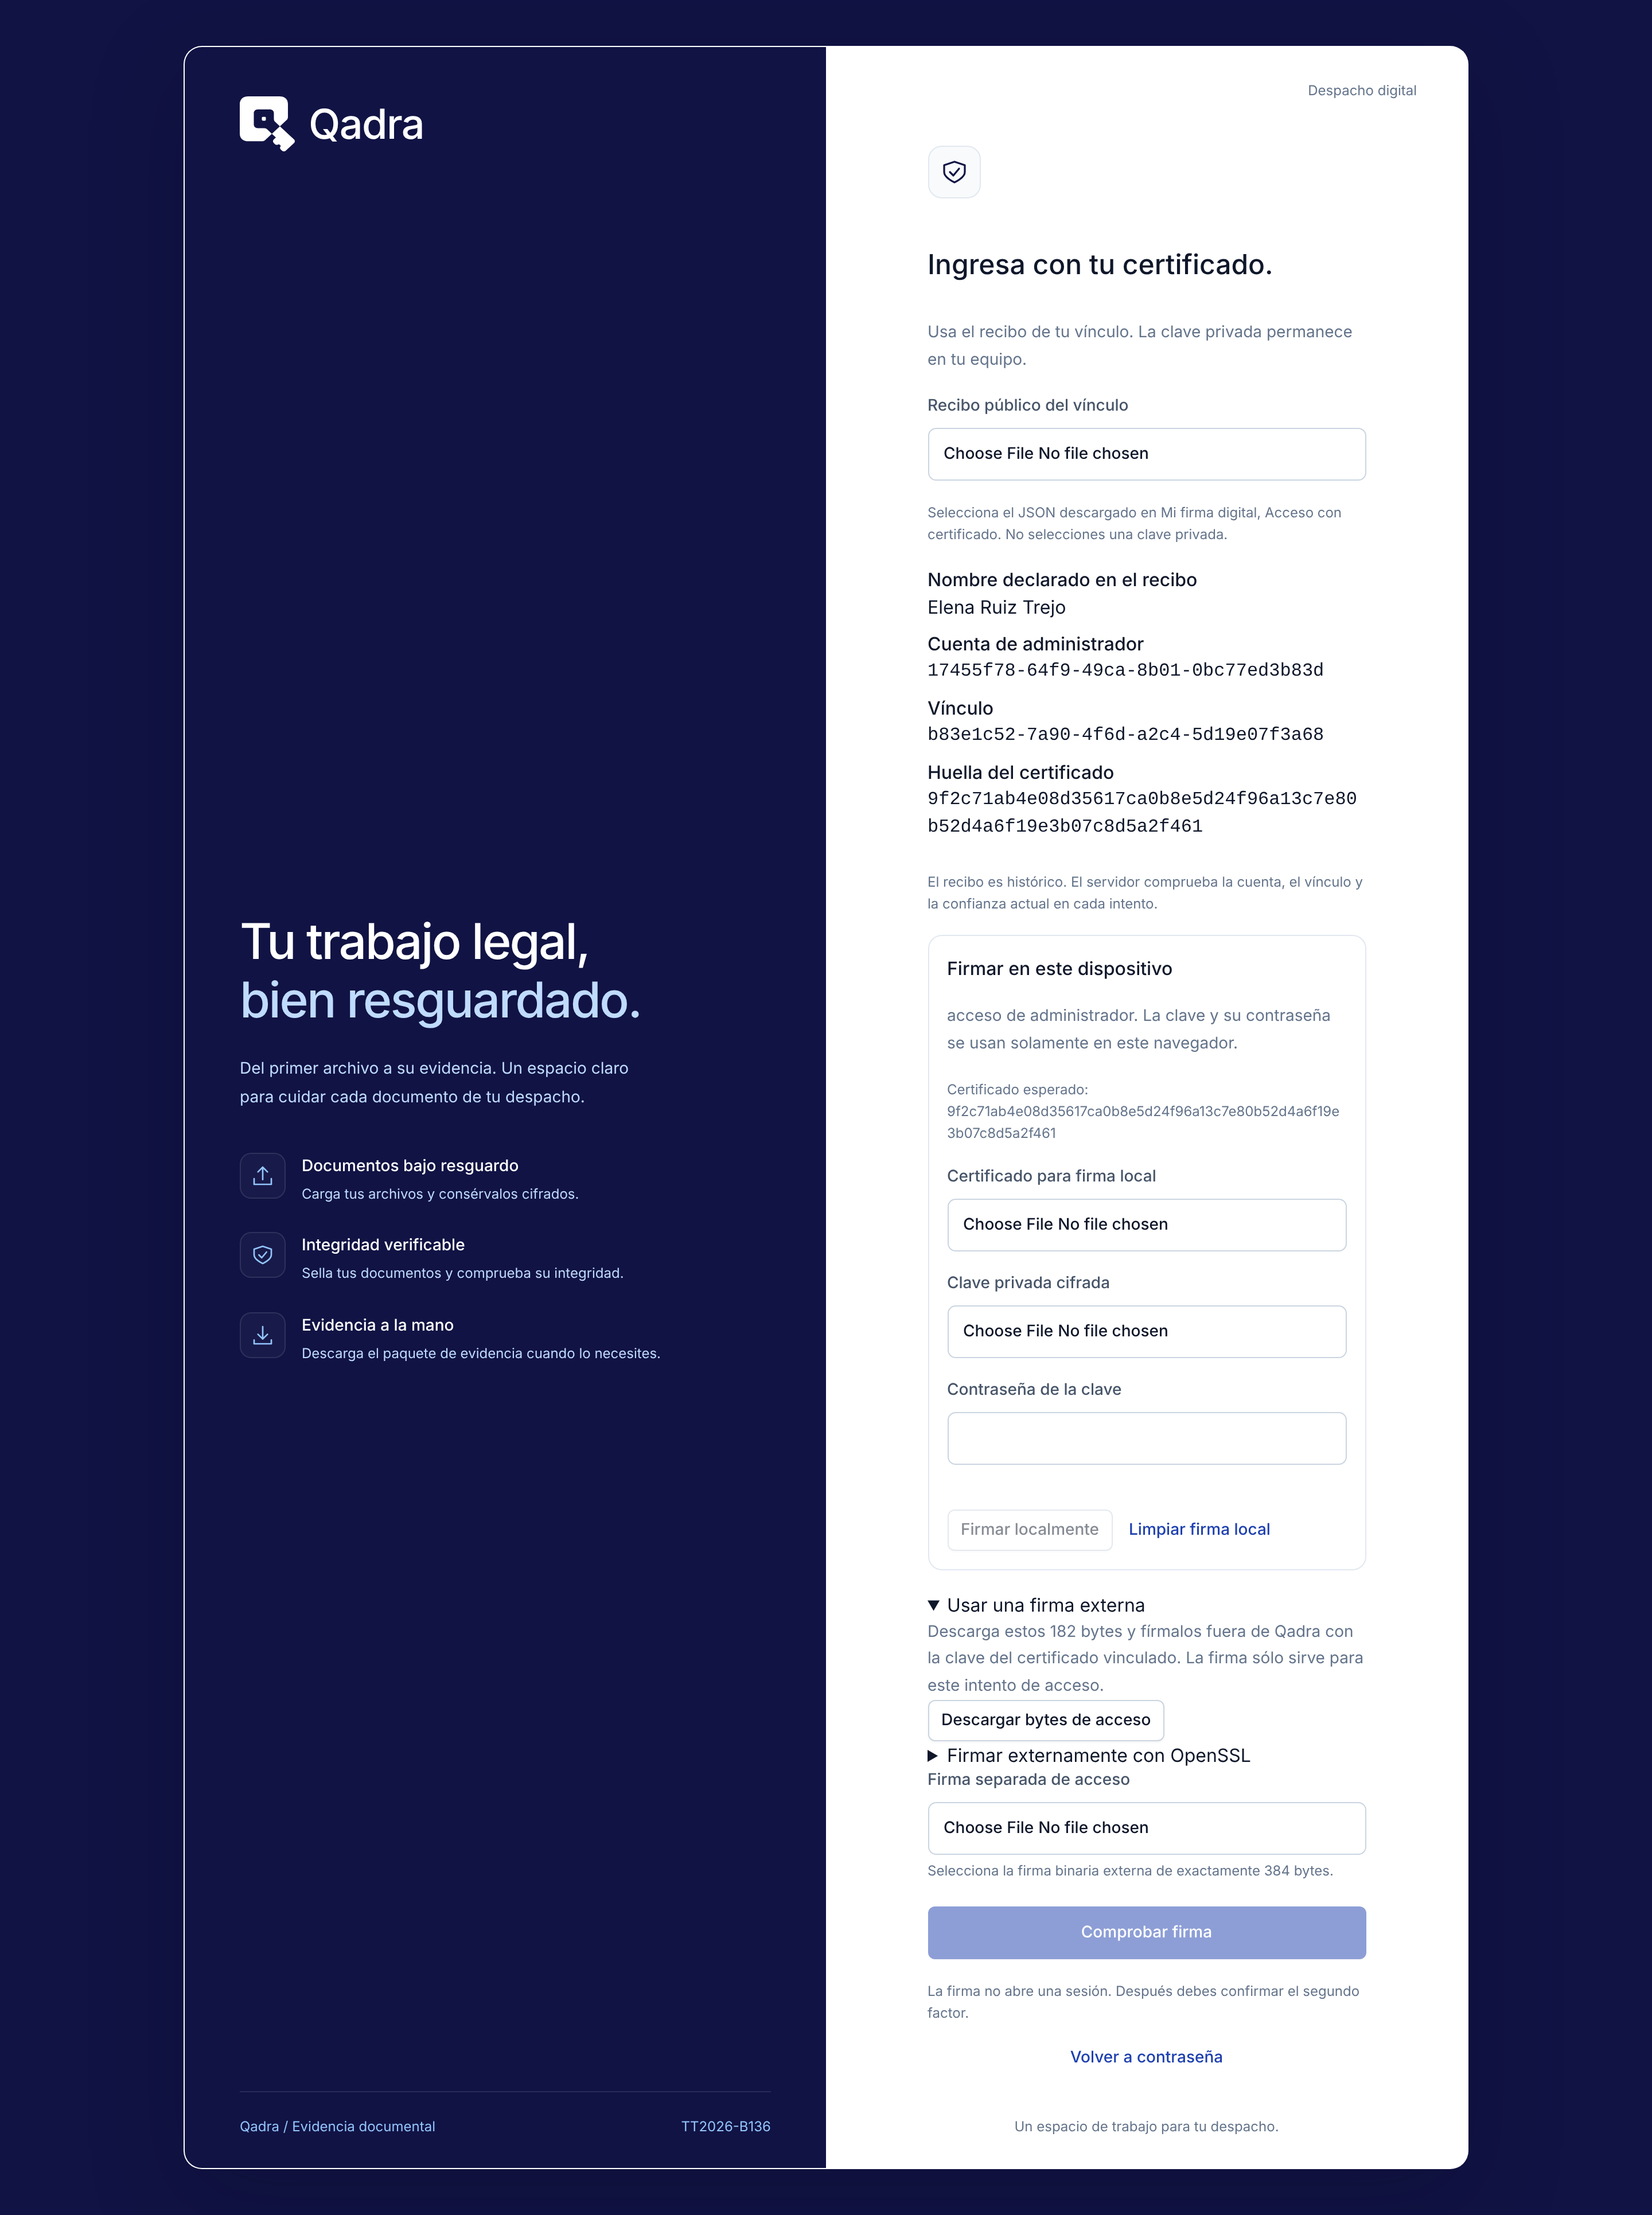
\includegraphics[width=0.9\textwidth]{capturas/A-09-ingresar-certificado.png}
  \caption{Inicio de sesión con certificado.}
  \label{fig:manual-ingresar-certificado}
\end{figure}

\resultado Se abre su espacio de trabajo como Administrador.

\begin{itemize}
  \item Su clave privada no sale de su equipo: la firma se hace en el
        navegador.
  \item Si prefiere firmar con su propia herramienta, abra
        \textbf{Usar una firma externa}, haga clic en
        \textbf{Descargar bytes de acceso}, firme el archivo
        \texttt{acceso-certificado.bin} y seleccione el resultado en
        \textbf{Firma separada de acceso}.
  \item Si tarda demasiado, aparece \enquote{El intento de acceso venció.
        Prepara otro intento y firma los nuevos bytes.} Haga clic en
        \textbf{Preparar otro intento}.
  \item Para volver al acceso normal, haga clic en
        \textbf{Volver a contraseña}.
\end{itemize}

% ---------------------------------------------------------------------
\section{Cerrar sesión y sesión terminada}\label{sec:cerrar-sesion}

\paraque Termina su sesión de forma segura cuando deja de trabajar.

\disponible Todos los roles con cuenta.

\pasos
\begin{enumerate}
  \item En la esquina superior derecha, haga clic en el círculo con sus
        iniciales (menú \textbf{Tu cuenta}).
  \item Revise su nombre, correo y rol, y haga clic en
        \textbf{Cerrar sesión}.
\end{enumerate}

\begin{figure}[H]
  \centering
  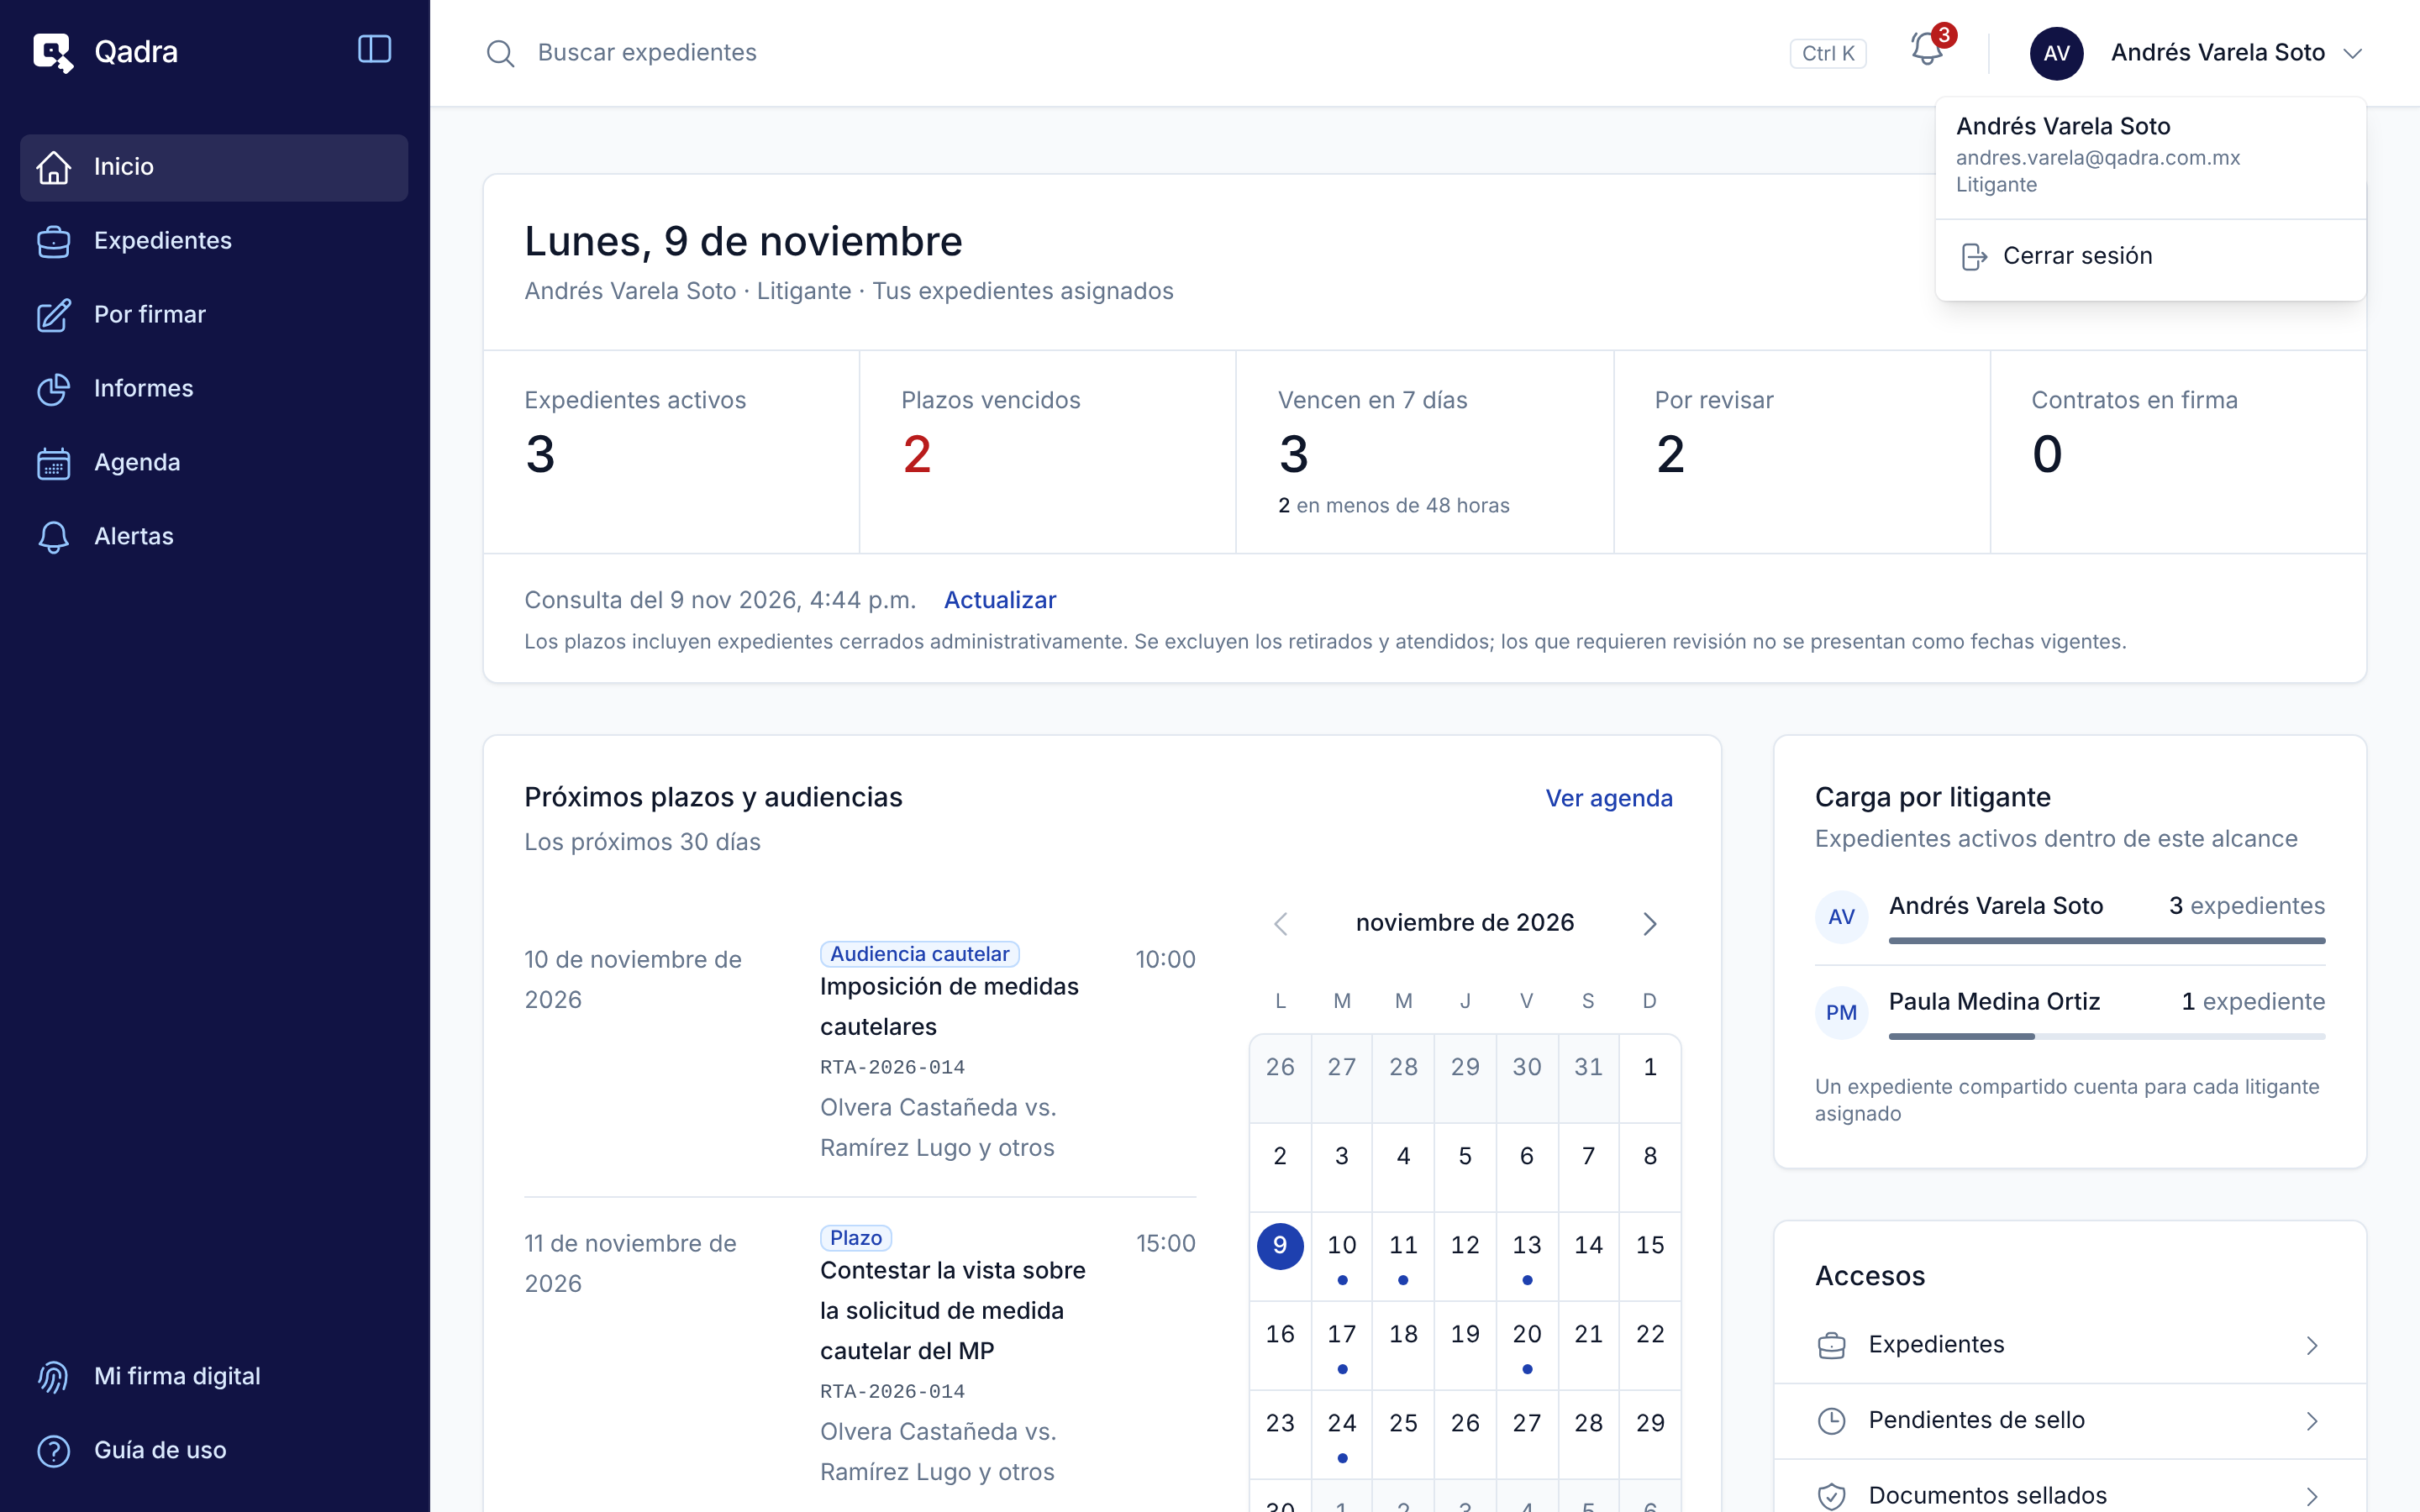
\includegraphics[width=0.9\textwidth]{capturas/A-10-menu-cuenta.png}
  \caption{Menú de la cuenta.}
  \label{fig:manual-menu-cuenta}
\end{figure}

\resultado Qadra vuelve a la pantalla de inicio de sesión.

\begin{itemize}
  \item \textbf{Sesión terminada:} si pasa mucho tiempo sin actividad, Qadra
        lo regresa al inicio de sesión con el mensaje \enquote{Tu sesión
        terminó. Vuelve a iniciar sesión.}
  \item \textbf{Al volver a la pestaña:} Qadra muestra \enquote{Comprobando
        tu sesión.} y conserva sus cambios en pantalla. Si no avanza, haga
        clic en \textbf{Comprobar de nuevo}.
  \item Si Qadra no pudo confirmar el cierre con el servidor, aparece
        \enquote{Saliste de esta pantalla. No se pudo confirmar el cierre en
        el servidor.} Cierre también la pestaña del navegador.
\end{itemize}
